\documentclass[11pt,a4paper]{article}

% --- Core LaTeX Packages ---
\usepackage[utf8]{inputenc}
\usepackage[T1]{fontenc}
\usepackage[scaled=0.95]{helvet}
\renewcommand{\familydefault}{\sfdefault}
\renewcommand{\ttdefault}{txtt}
\usepackage{upquote}
\usepackage[margin=0.85in, headheight=15pt]{geometry}
\usepackage{amsmath,amssymb,amsthm}
\usepackage[helvet]{sfmath}
\usepackage{microtype}
\DisableLigatures{encoding = *, family = tt*}
\usepackage{parskip}
\usepackage[table]{xcolor}
\usepackage{booktabs}
\usepackage{tabularx}
\usepackage{xltabular}
\usepackage{enumitem}
\usepackage{fancyhdr}
\usepackage[explicit]{titlesec}
\usepackage[skins,breakable]{tcolorbox}
\usepackage{listings}
\usepackage{hyperref}
\usepackage{graphicx}

% --- Diagram Packages ---
\usepackage{tikz}
\usetikzlibrary{arrows.meta,positioning,decorations.pathreplacing}

% --- Unified Print-Safe Color Palette ---
\definecolor{primaryblue}{RGB}{24, 75, 140}
\definecolor{accentteal}{RGB}{15, 118, 110}
\definecolor{accentamber}{RGB}{180, 83, 9}
\definecolor{accentred}{RGB}{185, 28, 28}
\definecolor{codebg}{RGB}{246, 248, 250}
\definecolor{codeframe}{RGB}{204, 212, 220}
\definecolor{codeink}{RGB}{24, 30, 38}
\definecolor{codekw}{RGB}{126, 34, 206}
\definecolor{codetype}{RGB}{0, 118, 138}
\definecolor{codegreen}{RGB}{22, 138, 66}
\definecolor{codeblue}{RGB}{15, 92, 212}
\definecolor{codestr}{RGB}{194, 65, 12}
\definecolor{codegray}{RGB}{105, 115, 125}

% --- Global Typography & Spacing ---
\linespread{1.08}
\renewcommand{\arraystretch}{1.32}
\setlength{\tabcolsep}{7pt}
\setlist[itemize]{itemsep=3pt, topsep=4pt, leftmargin=1.5em}
\setlist[enumerate]{itemsep=4pt, topsep=4pt, leftmargin=1.6em}

% --- Running Header & Footer (Screen + Print Navigation) ---
\pagestyle{fancy}
\fancyhf{}
\fancyhead[L]{\footnotesize\color{codegray}\textbf{Two Pointers \& Sliding Window}}
\fancyhead[R]{\footnotesize\color{codegray}\nouppercase{\leftmark}}
\fancyfoot[C]{\footnotesize\color{codegray}Page \thepage}
\renewcommand{\headrulewidth}{0.4pt}
\renewcommand{\headrule}{\hbox to\headwidth{\color{codeframe}\leaders\hrule height \headrulewidth\hfill}}
\renewcommand{\sectionmark}[1]{\markboth{\thesection.\ #1}{}}

% --- Section & Subsection Styling (High-Contrast + Per-Section Page Breaks) ---
\newcommand{\sectionbreak}{}

\titleformat{\section}[block]
  {\Large\bfseries\color{primaryblue}}
  {}
  {0pt}
  {\colorbox{primaryblue}{\color{white}\bfseries\Large\;\thesection\;}\hspace{0.55em}#1}
  [\vspace{4pt}{\color{primaryblue}\titlerule[1.4pt]}]
\titlespacing*{\section}{0pt}{4pt}{13pt}

\titleformat{name=\section,numberless}[block]
  {\Large\bfseries\color{primaryblue}}
  {}
  {0pt}
  {#1}
  [\vspace{4pt}{\color{primaryblue}\titlerule[1.4pt]}]

\titleformat{\subsection}[block]
  {\large\bfseries\color{primaryblue!90!black}}
  {}
  {0pt}
  {\begin{tcolorbox}[
      enhanced, colback=primaryblue!6, colframe=primaryblue!6,
      borderline west={3.5pt}{0pt}{primaryblue},
      sharp corners=west, arc=2pt,
      left=8pt, right=8pt, top=5pt, bottom=5pt,
      boxsep=0pt, before skip=0pt, after skip=0pt
  ]\large\bfseries\color{primaryblue!90!black}\thesubsection\hspace{0.55em}#1\end{tcolorbox}}
\titlespacing*{\subsection}{0pt}{16pt}{7pt}

\titleformat{name=\subsection,numberless}[block]
  {\normalsize\bfseries\color{accentteal}}
  {}
  {0pt}
  {#1}
  [\vspace{2pt}{\color{accentteal!40}\titlerule[0.7pt]}]
\titlespacing*{\subsection}{0pt}{13pt}{5pt}

% --- Canonical Shared TikZ Styles ---
\tikzset{
    lmbox/.style={draw=codeframe, fill=codebg, thick, rounded corners=2pt, inner sep=4pt, font=\small},
    lmactive/.style={draw=primaryblue, fill=primaryblue!8, thick, rounded corners=2pt, inner sep=4pt, font=\small\bfseries, text=primaryblue},
    lmaccepted/.style={draw=codegreen, fill=codegreen!10, thick, rounded corners=2pt, inner sep=4pt, font=\small\bfseries, text=codegreen},
    lmpruned/.style={draw=red!70!black, fill=red!70!black!6, thick, dashed, rounded corners=2pt, inner sep=4pt, font=\small, text=red!70!black},
    lmarrow/.style={-{Stealth[length=5pt]}, thick, primaryblue},
    lmmuted/.style={-{Stealth[length=5pt]}, thick, codegray},
    lmprunedarrow/.style={-{Stealth[length=5pt]}, thick, dashed, red!70!black}
}

% --- Hyperref Setup ---
\hypersetup{
    colorlinks=true,
    linkcolor=primaryblue,
    citecolor=primaryblue,
    urlcolor=primaryblue,
    pdftitle={Two Pointers and Sliding Window},
    pdfauthor={Antigravity Engineering}
}

% --- Example Environment ---
\theoremstyle{definition}
\newtheorem{example}{Example}[section]

% --- Semantic Narrative Beat Labels & Solution Trap Diagnostic ---
\newcommand{\painbeat}{\textbf{\color{accentamber}The Problem:} }
\newcommand{\ahabeat}{\textbf{\color{accentteal}The ``Aha!'' Insight:} }
\newcommand{\examplebeat}{\textbf{\color{primaryblue}Mini-Example First:} }
\newcommand{\breaksbeat}{\textbf{\color{accentred}When It Breaks:} }
\newcommand{\invariantbeat}[1]{\par\noindent\textbf{\color{accentteal}Loop Invariant (#1):} }
\newcommand{\trapnote}[1]{\par\smallskip\noindent{\footnotesize\textbf{\color{accentamber}Common trap:} #1}}

% --- Modern Overview Card ---
\newtcolorbox{overviewbox}[1][What You'll Learn]{
    enhanced,
    colback=accentteal!5, colframe=accentteal!25,
    borderline west={3.5pt}{0pt}{accentteal},
    arc=3pt, boxrule=0.5pt,
    left=10pt, right=10pt, top=7pt, bottom=7pt,
    fonttitle=\bfseries\color{accentteal},
    title={#1},
    attach title to upper={\par\vspace{2pt}}
}

% --- Key Takeaway / Core Rule Box ---
\newtcolorbox{calloutbox}[1]{
    enhanced,
    colback=accentteal!5, colframe=accentteal!25,
    borderline west={3.5pt}{0pt}{accentteal},
    arc=3pt, boxrule=0.5pt,
    left=10pt, right=10pt, top=7pt, bottom=7pt,
    before skip=8pt, after skip=8pt,
    fonttitle=\bfseries\color{accentteal},
    title={#1},
    attach title to upper={\par\vspace{3pt}}
}

% --- Plain-English Formula Card ---
\newtcolorbox{formulabox}[1][Formula in Plain English]{
    enhanced,
    colback=primaryblue!4, colframe=primaryblue!22,
    borderline west={3.5pt}{0pt}{primaryblue},
    arc=3pt, boxrule=0.5pt,
    left=10pt, right=10pt, top=6pt, bottom=6pt,
    before skip=8pt, after skip=8pt,
    fonttitle=\small\bfseries\color{primaryblue},
    title={#1},
    attach title to upper={\par\vspace{2pt}}
}

% --- Watch-Out / Edge-Case Warning Box ---
\newtcolorbox{watchoutbox}[1][Watch Out --- When It Breaks]{
    enhanced,
    colback=accentamber!6, colframe=accentamber!30,
    borderline west={3.5pt}{0pt}{accentamber},
    arc=3pt, boxrule=0.5pt,
    left=10pt, right=10pt, top=7pt, bottom=7pt,
    before skip=8pt, after skip=8pt,
    fonttitle=\bfseries\color{accentamber},
    title={#1},
    attach title to upper={\par\vspace{3pt}}
}

% --- Local Symbol Mini-Table Environment ---
\newenvironment{notationbox}[1][Symbols Used Here]{
    \par\vspace{0.15cm}
    \noindent\textbf{\small\color{primaryblue}#1}\par\vspace{0.1cm}
    \begingroup
    \footnotesize
    \rowcolors{2}{codebg}{white}
    \noindent\tabularx{\textwidth}{>{\raggedright\arraybackslash\bfseries}l >{\raggedright\arraybackslash}X >{\raggedright\arraybackslash}p{3.8cm}}
    \arrayrulecolor{primaryblue}\toprule[1.1pt]
    \rowcolor{primaryblue!10}
    \textcolor{primaryblue}{\textbf{Symbol}} & \textcolor{primaryblue}{\textbf{Plain-English Meaning}} & \textcolor{primaryblue}{\textbf{Example / Type}} \\
    \arrayrulecolor{codeframe}\midrule[0.6pt]
}{
    \arrayrulecolor{primaryblue}\bottomrule[1.1pt]
    \endtabularx
    \endgroup
    \vspace{0.2cm}\par
}

% --- Print-First Pen-and-Paper Exercise Environment ---
\newcounter{exercise}
\newtcolorbox{tryitbox}[3]{
    enhanced,
    step=exercise,
    colback=codegreen!3, colframe=codegreen!45,
    colbacktitle=codegreen!14, coltitle=codegreen!85!black,
    borderline west={3.5pt}{0pt}{codegreen},
    arc=3pt, boxrule=0.6pt,
    left=10pt, right=10pt, top=7pt, bottom=7pt,
    toptitle=4pt, bottomtitle=4pt,
    before skip=9pt, after skip=9pt,
    fonttitle=\bfseries,
    title={Exercise \theexercise\hspace{0.5em}{\colorbox{codegreen!85!black}{\color{white}\scriptsize\bfseries\;#1\;}}\hspace{0.5em}#2 \hfill {\normalfont\footnotesize\color{codegray}Answer: p.~\pageref*{sol:#3}}}
}

% --- Modern C++23 Code Listing Setup ---
\lstset{
    language=C++,
    basicstyle=\small\ttfamily\color{codeink},
    keywordstyle=\color{codekw}\bfseries,
    morekeywords={constexpr,noexcept,nullptr,static_assert,auto,override,final,decltype,concept,requires},
    keywordstyle=[2]\color{codetype}\bfseries,
    morekeywords=[2]{std,vector,span,deque,string,string_view,size_t,int64_t,uint32_t,uint64_t,optional,pair,tuple,array,priority_queue,unordered_map,unordered_set,map,set,ranges,views,nodiscard},
    moredelim=[l][\color{codeblue}\bfseries]{\#},
    deletestring=[b]',
    commentstyle=\color{codegreen}\itshape,
    stringstyle=\color{codestr},
    numberstyle=\tiny\color{codegray},
    numbers=left,
    numbersep=8pt,
    xleftmargin=24pt,
    framexleftmargin=22pt,
    framexrightmargin=4pt,
    framextopmargin=4pt,
    framexbottommargin=4pt,
    backgroundcolor=\color{codebg},
    frame=single,
    rulecolor=\color{codeframe},
    aboveskip=8pt,
    belowskip=10pt,
    breaklines=true,
    breakatwhitespace=true,
    tabsize=4,
    showstringspaces=false,
    captionpos=b
}

\begin{document}

% --- Modern Title Banner ---
\thispagestyle{plain}
\begin{tcolorbox}[
    enhanced,
    colback=primaryblue!6, colframe=primaryblue!20,
    borderline west={5pt}{0pt}{primaryblue},
    arc=4pt, boxrule=0.6pt,
    left=14pt, right=14pt, top=7pt, bottom=7pt,
    before skip=0pt, after skip=5pt
]
    {\footnotesize\bfseries\color{accentteal}MODULE 13 \quad|\quad ALGORITHMS \& DATA STRUCTURES STUDY GUIDE}\\[3pt]
    {\Huge\bfseries\color{primaryblue}Two Pointers \& Sliding Window}\\[3pt]
    {\large\color{codegray}Collapsing Quadratic $O(N^2)$ Nested Loops into Single-Pass Linear Scans}\\[4pt]
    {\footnotesize\color{codegray}Updated \today}
\end{tcolorbox}

\begin{overviewbox}[What You'll Learn]
{\small Many array and string problems invite an obvious nested loop over all pairs $(i, j)$ or all contiguous subarrays $[L, R]$, costing $O(N^2)$ time and timing out at $N = 10^5$. This guide shows how two coordinated indices collapse those searches to $O(N)$ by never retreating: opposite-direction pointers (pair sums, 3-Sum, Container With Most Water), fast/slow pointers (in-place deduplication, Dutch National Flag, Floyd's cycle entry proof), and fixed, variable, and ``at most $K$'' sliding windows --- plus exactly when negative numbers break the window invariant.}
\end{overviewbox}

\vspace{-6pt}
{\setlength{\parskip}{0pt}\footnotesize
\titlespacing*{\section}{0pt}{2pt}{6pt}%
\makeatletter
\let\lm@orig@addvspace\addvspace
\renewcommand{\addvspace}[1]{\lm@orig@addvspace{0.18em plus 1pt}}
\makeatother
\tableofcontents}

% Every major section starts cleanly on a new page
\renewcommand{\sectionbreak}{\clearpage}

% ============================================================================
\section{Foundations: Turning Quadratic Loops into Linear Scans}
% ============================================================================

Whenever a problem asks about pairs of elements $(i, j)$ or contiguous subarrays $A[L \dots R]$, the brute-force instinct is two nested loops: fix $i$, then scan every $j > i$. On an array of $N = 10^5$ elements, $\binom{N}{2} \approx 5 \times 10^9$ iterations take tens of seconds.

Two-pointer and sliding-window techniques eliminate that inner rescan. Instead of restarting the second index from scratch every time the first index moves, you maintain a \textbf{monotonic state} so both indices move forward (or inward) without ever backing up.

\subsection{Three Pointer Geometries at a Glance}

Almost every linear-pass array or string algorithm falls into one of three geometric layouts:

\begingroup\small\rowcolors{2}{codebg}{white}
\begin{tabularx}{\textwidth}{>{\raggedright\arraybackslash\bfseries}p{3.6cm} >{\raggedright\arraybackslash}p{3.5cm} >{\raggedright\arraybackslash}X}
\arrayrulecolor{primaryblue}\toprule[1.2pt]
\rowcolor{primaryblue!10}
\textcolor{primaryblue}{\textbf{Geometry}} & \textcolor{primaryblue}{\textbf{Pointer Motion}} & \textcolor{primaryblue}{\textbf{Real-World Analogy \& Core Use}} \\
\arrayrulecolor{codeframe}\midrule[0.6pt]
Opposite-Direction (Converging) & $L$ starts at $0$ ($\to$); $R$ starts at $N-1$ ($\leftarrow$); stop at $L \ge R$. & Two fingers scanning a sorted ledger from both ends toward the middle. Pair sums, 3-Sum, area maximization, palindrome checks. \\
Fast \& Slow (Same-Direction) & Both start at $0$ ($\to$); \texttt{fast} moves ahead of \texttt{slow} (read/write or $2\times$ speed). & A fast runner lapping a slow runner on a track, or a reader copying valid items into a compact buffer. In-place deduplication, partitioning, cycle detection. \\
Sliding Window $[L, R]$ & Both start at $0$ ($\to$); $R$ expands the window, $L$ shrinks it. & A magnifying glass gliding across an audio waveform without restarting at the left edge. Fixed-length sums, shortest/longest valid subarrays, exact-$K$ counting. \\
\arrayrulecolor{primaryblue}\bottomrule[1.2pt]
\end{tabularx}\endgroup

\subsection{Why a Nested \texttt{while} Loop Is Still $O(N)$}

Beginners often see a \texttt{while} loop nested inside a \texttt{for} loop and assume the worst-case time must be $O(N^2)$. That assumption is wrong whenever the inner pointer never resets.

\begin{formulabox}[The Monotonic Pointer Budget (Amortized $O(N)$)]
$$\text{Total pointer moves} \;=\; (\#\text{ of } R\text{ steps}) + (\#\text{ of } L\text{ steps}) \;\le\; N + N \;=\; 2N \;=\; O(N).$$
\textbf{Read this as:} Even if one single outer step triggers $50{,}000$ inner shrinks of $L$, those $50{,}000$ elements are evicted \emph{permanently}. Across the entire run of the algorithm, each index $0, 1, \dots, N-1$ enters the window at most once (when $R$ passes it) and leaves at most once (when $L$ passes it).
\end{formulabox}

Think of it as a prepaid transit card with $2N$ tokens: every increment of $R$ or $L$ spends $1$ token, and because neither pointer ever moves backward, you can never spend more than $2N$ tokens in total. If each step updates window state in $O(1)$ time, the whole algorithm runs in $O(N)$.

\begingroup\small\rowcolors{2}{codebg}{white}
\begin{tabularx}{\textwidth}{>{\raggedright\arraybackslash\bfseries}p{4.1cm} >{\centering\arraybackslash}p{2.2cm} >{\centering\arraybackslash}p{2.2cm} >{\raggedright\arraybackslash}X}
\arrayrulecolor{primaryblue}\toprule[1.2pt]
\rowcolor{primaryblue!10}
\textcolor{primaryblue}{\textbf{Task}} & \textcolor{primaryblue}{\textbf{Naive Loop}} & \textcolor{primaryblue}{\textbf{Two Pointers}} & \textcolor{primaryblue}{\textbf{What Was Eliminated}} \\
\arrayrulecolor{codeframe}\midrule[0.6pt]
Sorted Pair Sum & $O(N^2)$ & $O(N)$ & Eliminating an entire row or column per comparison. \\
Remove Duplicates In-Place & $O(N^2)$ & $O(N)$ & Repeated left-shifts after every \texttt{vector::erase}. \\
Fixed Window Sum ($K$) & $O(N \cdot K)$ & $O(N)$ & Re-summing $K - 1$ overlapping elements each shift. \\
Shortest Subarray Sum $\ge S$ & $O(N^2)$ & $O(N)$ & Restarting $R$ from $L$ whenever $L$ advances (for $A[i] \ge 0$). \\
\arrayrulecolor{primaryblue}\bottomrule[1.2pt]
\end{tabularx}\endgroup

\begin{tryitbox}{Derive}{Proving the Amortized Movement Budget}{ex1}
Suppose a sliding window uses indices $L$ and $R$ over an array of length $N \ge 1$. Initially $L = 0$ and $R$ loops from $0$ to $N - 1$. Inside the loop, $L$ only increments while $L \le R$ (and never decrements).
\begin{enumerate}[itemsep=2pt, topsep=2pt]
    \item What is the exact maximum number of times the inner \texttt{L++} statement can execute across the \emph{entire} program?
    \item Suppose instead a programmer resets \texttt{L = 0} whenever the window becomes empty, or resets \texttt{R = L} whenever the window becomes invalid. Construct a tiny worst-case behavior and state the new time complexity.
\end{enumerate}
\end{tryitbox}

% ============================================================================
\section{Opposite-Direction (Converging) Pointers}
% ============================================================================

Opposite-direction pointers start at the two extremes of an array ($L = 0$ and $R = N - 1$) and walk inward until they meet ($L \ge R$). At every step, a single $O(1)$ comparison proves that \textbf{all remaining partners} of either $L$ or $R$ can be safely discarded.

\begin{notationbox}[Symbols Used in Converging Pointers]
$L, R$ & Left and right inclusive indices moving inward ($0 \le L < R < N$). & \texttt{std::size\_t} \\
$A[i],\, h[i]$ & Array value (sorted) or vertical wall height at index $i$. & \texttt{int} / \texttt{int64\_t} \\
$T$ & Target pair sum (or $0$ in Three-Sum). & \texttt{int64\_t} \\
$\text{area}(L, R)$ & Water held between walls $L$ and $R$: $(R - L) \cdot \min(h[L], h[R])$. & \texttt{int64\_t} \\
\end{notationbox}

\subsection{Sorted Pair Sum (Row-and-Column Elimination)}

\painbeat Given a sorted array $A$ of $N$ integers and a target $T$, find indices $L < R$ with $A[L] + A[R] = T$. Checking all $\binom{N}{2}$ pairs takes $O(N^2)$ time, and binary searching $T - A[i]$ for each $i$ still takes $O(N \log N)$.

\ahabeat Because $A$ is sorted in non-decreasing order, comparing the \emph{extreme} pair $A[L] + A[R]$ against $T$ rules out an entire batch of pairs in one step. Look at the $N \times N$ table of all pair sums $A[i] + A[j]$: every row increases left-to-right and every column increases top-to-bottom.

\examplebeat Let $A = [1, 3, 4, 6, 8, 11]$ and $T = 10$. Start at $(L, R) = (0, 5)$:
\begin{enumerate}[itemsep=2pt, topsep=2pt]
    \item $A[0] + A[5] = 1 + 11 = 12 > 10$. Since $1$ is the \emph{smallest} element left, pairing $11$ with anything right of $1$ gives an even larger sum! So $11$ can never be part of the answer $\implies R \leftarrow 4$.
    \item $A[0] + A[4] = 1 + 8 = 9 < 10$. Since $8$ is the \emph{largest} element left, pairing $1$ with anything left of $8$ gives an even smaller sum! So $1$ is dead $\implies L \leftarrow 1$.
    \item $A[1] + A[4] = 3 + 8 = 11 > 10 \implies R \leftarrow 3$.
    \item $A[1] + A[3] = 3 + 6 = 9 < 10 \implies L \leftarrow 2$.
    \item $A[2] + A[3] = 4 + 6 = 10 = T \implies$ \textbf{Match found at $(2, 3)$!}
\end{enumerate}

\begin{formulabox}[Sorted Pair Elimination Rule]
For sorted $A$ with current bounds $L < R$:
\begin{itemize}[itemsep=1pt, topsep=2pt]
    \item If $A[L] + A[R] < T$, then $A[L] + A[j] \le A[L] + A[R] < T$ for every $j \in [L+1, R]$ $\implies$ discard $L$ (\texttt{L++}).
    \item If $A[L] + A[R] > T$, then $A[i] + A[R] \ge A[L] + A[R] > T$ for every $i \in [L, R-1]$ $\implies$ discard $R$ (\texttt{R--}).
\end{itemize}
\textbf{Read this as:} Each step deletes either the top remaining row or the rightmost remaining column of the pair-sum matrix, so the pointers meet in at most $N - 1$ steps.
\end{formulabox}

\begin{figure}[htbp]
\centering
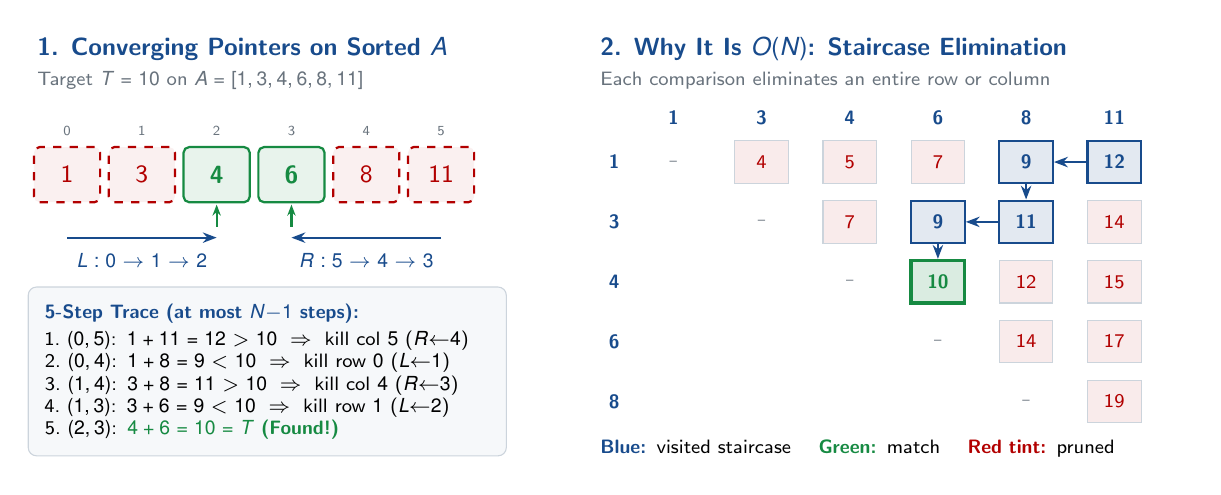
\begin{tikzpicture}[
    cell/.style={draw=codeframe, minimum width=0.68cm, minimum height=0.54cm, font=\scriptsize, inner sep=0pt, align=center}
]
    % === Left Panel: Sorted Array & Converging Pointers (x = 0.0 .. 6.0) ===
    \node[font=\small\bfseries\color{primaryblue}, anchor=west] at (0.0, 5.10) {1. Converging Pointers on Sorted $A$};
    \node[font=\scriptsize\color{codegray}, anchor=west] at (0.0, 4.70) {Target $T = 10$ on $A = [1, 3, 4, 6, 8, 11]$};

    \foreach \val/\idx/\sty in {1/0/lmpruned, 3/1/lmpruned, 4/2/lmaccepted, 6/3/lmaccepted, 8/4/lmpruned, 11/5/lmpruned} {
        \node[\sty, minimum width=0.84cm, minimum height=0.70cm, inner sep=0pt] (a\idx) at (0.50 + \idx*0.95, 3.50) {\val};
        \node[font=\tiny\color{codegray}] at (0.50 + \idx*0.95, 4.06) {\idx};
    }

    % Pointer trajectories
    \draw[lmarrow] (0.50, 2.70) -- (2.40, 2.70) node[midway, below=2pt, font=\scriptsize\color{primaryblue}] {$L: 0 \to 1 \to 2$};
    \draw[lmarrow] (5.25, 2.70) -- (3.35, 2.70) node[midway, below=2pt, font=\scriptsize\color{primaryblue}] {$R: 5 \to 4 \to 3$};
    \draw[thick, codegreen, -{Stealth[length=4pt]}] (2.40, 2.84) -- (2.40, 3.12);
    \draw[thick, codegreen, -{Stealth[length=4pt]}] (3.35, 2.84) -- (3.35, 3.12);

    % Step ledger card
    \node[draw=codeframe, fill=codebg, rounded corners=3pt, text width=5.65cm, inner sep=6pt, font=\scriptsize, anchor=north west] at (0.0, 2.08) {
        \textbf{\color{primaryblue}5-Step Trace (at most $N{-}1$ steps):}\\[2pt]
        1.\ $(0,5)$: $1+11=12 > 10 \;\Rightarrow\; \text{kill col } 5$ ($R{\leftarrow}4$)\\
        2.\ $(0,4)$: $1+8=9 < 10 \;\Rightarrow\; \text{kill row } 0$ ($L{\leftarrow}1$)\\
        3.\ $(1,4)$: $3+8=11 > 10 \;\Rightarrow\; \text{kill col } 4$ ($R{\leftarrow}3$)\\
        4.\ $(1,3)$: $3+6=9 < 10 \;\Rightarrow\; \text{kill row } 1$ ($L{\leftarrow}2$)\\
        5.\ $(2,3)$: \textbf{\color{codegreen}$4+6=10 = T$ (Found!)}
    };

    % === Right Panel: Upper-Triangular Pair-Sum Matrix (x = 7.1 .. 14.9) ===
    \node[font=\small\bfseries\color{primaryblue}, anchor=west] at (7.15, 5.10) {2. Why It Is $O(N)$: Staircase Elimination};
    \node[font=\scriptsize\color{codegray}, anchor=west] at (7.15, 4.70) {Each comparison eliminates an entire row or column};

    % Column headers (j = 0..5): x = 8.20 + j*1.12 -> rightmost center 13.80, edge 14.14
    \foreach \val/\j in {1/0, 3/1, 4/2, 6/3, 8/4, 11/5} {
        \node[font=\scriptsize\bfseries\color{primaryblue}] at (8.20 + \j*1.12, 4.22) {\val};
    }
    % Row headers (i = 0..4)
    \foreach \val/\i in {1/0, 3/1, 4/2, 6/3, 8/4} {
        \node[font=\scriptsize\bfseries\color{primaryblue}] at (7.45, 3.66 - \i*0.76) {\val};
    }

    % Row 0 (A[0]=1)
    \node[cell, fill=red!70!black!8, text=red!70!black] (m01) at (8.20 + 1*1.12, 3.66) {4};
    \node[cell, fill=red!70!black!8, text=red!70!black] (m02) at (8.20 + 2*1.12, 3.66) {5};
    \node[cell, fill=red!70!black!8, text=red!70!black] (m03) at (8.20 + 3*1.12, 3.66) {7};
    \node[cell, fill=primaryblue!12, draw=primaryblue, thick, text=primaryblue] (m04) at (8.20 + 4*1.12, 3.66) {\textbf{9}};
    \node[cell, fill=primaryblue!12, draw=primaryblue, thick, text=primaryblue] (m05) at (8.20 + 5*1.12, 3.66) {\textbf{12}};

    % Row 1 (A[1]=3)
    \node[cell, fill=red!70!black!8, text=red!70!black] (m12) at (8.20 + 2*1.12, 3.66 - 0.76) {7};
    \node[cell, fill=primaryblue!12, draw=primaryblue, thick, text=primaryblue] (m13) at (8.20 + 3*1.12, 3.66 - 0.76) {\textbf{9}};
    \node[cell, fill=primaryblue!12, draw=primaryblue, thick, text=primaryblue] (m14) at (8.20 + 4*1.12, 3.66 - 0.76) {\textbf{11}};
    \node[cell, fill=red!70!black!8, text=red!70!black] (m15) at (8.20 + 5*1.12, 3.66 - 0.76) {14};

    % Row 2 (A[2]=4)
    \node[cell, fill=codegreen!16, draw=codegreen, very thick, text=codegreen] (m23) at (8.20 + 3*1.12, 3.66 - 1.52) {\textbf{10}};
    \node[cell, fill=red!70!black!8, text=red!70!black] (m24) at (8.20 + 4*1.12, 3.66 - 1.52) {12};
    \node[cell, fill=red!70!black!8, text=red!70!black] (m25) at (8.20 + 5*1.12, 3.66 - 1.52) {15};

    % Row 3 (A[3]=6)
    \node[cell, fill=red!70!black!8, text=red!70!black] (m34) at (8.20 + 4*1.12, 3.66 - 2.28) {14};
    \node[cell, fill=red!70!black!8, text=red!70!black] (m35) at (8.20 + 5*1.12, 3.66 - 2.28) {17};

    % Row 4 (A[4]=8)
    \node[cell, fill=red!70!black!8, text=red!70!black] (m45) at (8.20 + 5*1.12, 3.66 - 3.04) {19};

    % Diagonal placeholders (i >= j)
    \foreach \i in {0,1,2,3,4} {
        \node[font=\tiny\color{codegray}] at (8.20 + \i*1.12, 3.66 - \i*0.76) {--};
    }

    % Staircase walk arrows (crisp 0.44cm horizontal / 0.22cm vertical clearance)
    \draw[lmarrow] (m05.west) -- (m04.east);
    \draw[lmarrow] (m04.south) -- (m14.north);
    \draw[lmarrow] (m14.west) -- (m13.east);
    \draw[lmarrow] (m13.south) -- (m23.north);

    % Compact legend neatly inside right panel width
    \node[font=\scriptsize, anchor=north west, text width=7.4cm] at (7.15, 0.25) {
        \textcolor{primaryblue}{\textbf{Blue:}} visited staircase \quad
        \textcolor{codegreen}{\textbf{Green:}} match \quad
        \textcolor{red!70!black}{\textbf{Red tint:}} pruned
    };
\end{tikzpicture}
\caption{Converging two pointers walk a single monotonic staircase across the upper-triangular pair-sum matrix, visiting at most $N - 1$ cells instead of all $\binom{N}{2}$.}
\label{fig:converging_grid}
\end{figure}

\begin{watchoutbox}[Watch Out --- Unsorted Input Destroys Elimination]
If $A$ is \textbf{not} sorted, observing $A[L] + A[R] < T$ proves nothing: a larger value might sit at $R - 1$. On unsorted input, either sort first in $O(N \log N)$ (if original indices are not needed, or pair values with original indices) or use a hash map in $O(N)$ time and $O(N)$ space.
\end{watchoutbox}

\begin{tryitbox}{Trace}{Converging Pair Sum}{ex2}
Hand-trace converging two pointers on the sorted array $A = [2, 5, 7, 9, 12, 15]$ with target $T = 16$. At each step record $(L, R)$, $A[L] + A[R]$, which row or column is eliminated, and which pointer moves.
\end{tryitbox}

\subsection{Three-Sum and Duplicate Skipping}

\painbeat Finding all \emph{unique} triplets $(A[i], A[j], A[k])$ with $i < j < k$ and $A[i] + A[j] + A[k] = 0$ takes $O(N^3)$ naively, and inserting sorted triplets into a hash set adds heavy constant factors and $O(N^2)$ memory.

\ahabeat Sort $A$ first in $O(N \log N)$. Fix the first number $A[i]$ in an outer loop, then solve \textbf{Sorted Pair Sum} on the suffix $A[i+1 \dots N-1]$ for target $-A[i]$ in $O(N)$ time --- dropping total runtime from $O(N^3)$ to $O(N^2)$ with $O(1)$ extra space (ignoring the output and sort stack).

Sorting also solves duplicate elimination cleanly with two simple guards:
\begin{enumerate}[itemsep=2pt, topsep=2pt]
    \item \textbf{Outer skip:} If $i > 0$ and $A[i] = A[i - 1]$, skip $i$ because every valid triplet starting with value $A[i]$ was already found when $i - 1$ was processed.
    \item \textbf{Inner skip (only \emph{after} recording a match):} After recording $(A[i], A[L], A[R])$, advance $L$ while $L < R$ and $A[L] = A[L - 1]$, and retreat $R$ while $L < R$ and $A[R] = A[R + 1]$.
    \item \textbf{Early stop:} Because $A$ is sorted, if $A[i] > 0$, then $A[i] + A[L] + A[R] \ge 3 A[i] > 0$, so break out immediately.
\end{enumerate}

\begin{watchoutbox}[Watch Out --- Never Skip Forward Before Checking]
Writing \texttt{if (A[i] == A[i + 1]) continue;} is a classic bug. On $[-1, -1, 2]$, skipping the \emph{first} $-1$ jumps to $i = 1$, leaving only $[-1, 2]$ and missing the valid triplet $(-1, -1, 2)$. Always compare against the \textbf{previous} index ($i - 1$) so the first copy of a repeated value still sees all later duplicates as candidates for $L$ and $R$.
\end{watchoutbox}

\subsection{Container With Most Water (Greedy Dominance Proof)}

\painbeat Given $N$ vertical walls of heights $h[0 \dots N-1]$, pick two walls $L < R$ to maximize the trapped water area $\text{area}(L, R) = (R - L) \cdot \min(h[L], h[R])$. The array $h$ is \emph{not} sorted, yet we still want $O(N)$ time.

\ahabeat Start at the widest possible container $(L, R) = (0, N - 1)$. Suppose $h[L] \le h[R]$ (the left wall is the bottleneck). Could keeping $L$ and pairing it with any interior wall $j \in (L, R)$ ever beat $(L, R)$? No! Moving $R$ inward strictly shrinks the width ($j - L < R - L$), while the water height stays capped at $\min(h[L], h[j]) \le h[L]$.

\begin{formulabox}[Shorter-Wall Dominance Inequality]
If $h[L] \le h[R]$, then for \textbf{every} interior wall $j \in \{L+1, \dots, R-1\}$:
$$\text{area}(L, j) \;=\; (j - L) \cdot \min(h[L], h[j]) \;<\; (R - L) \cdot h[L] \;=\; \text{area}(L, R).$$
\textbf{Read this as:} Once we record $\text{area}(L, R)$, the shorter wall $L$ has achieved its \emph{absolute maximum possible} area with any partner inside $[L, R]$. Discarding the shorter wall never discards an optimal solution.
\end{formulabox}

What if $h[L] = h[R]$? The exact same inequality applies symmetrically to \emph{both} walls: neither $(L, j)$ nor $(i, R)$ can exceed $(R - L) \cdot h[L]$! So advancing $L$ (or retreating $R$, or even moving both at once) is 100\% safe.

\begin{watchoutbox}[Watch Out --- Moving the Taller Wall Loses the Optimum]
On $h = [1, 8, 2, 3]$, starting at $(0, 3)$ gives area $3 \cdot \min(1, 3) = 3$. If you wrongly move the \emph{taller} wall ($R \leftarrow 2$), you check $(0, 2) = 2$ and $(0, 1) = 1$, returning $3$ and completely missing the true optimum $(1, 3)$ of area $2 \cdot \min(8, 3) = 6$.
\end{watchoutbox}

\begin{tryitbox}{Debug}{Breaking a Plausible Neighbor-Peek Heuristic}{ex3}
A teammate proposes a ``smarter'' rule for Container With Most Water: instead of always moving the shorter wall, compare the \emph{next} walls $h[L + 1]$ and $h[R - 1]$ and advance whichever side steps onto a taller neighbor (tie-breaking by \texttt{R--}).
\begin{enumerate}[itemsep=2pt, topsep=2pt]
    \item Trace this buggy rule on $h = [1, 2, 10, 10, 1]$. What maximum area does it report?
    \item What is the true maximum area on $h = [1, 2, 10, 10, 1]$, and why did the shorter-wall rule find it?
\end{enumerate}
\end{tryitbox}

% ============================================================================
\section{Same-Direction Fast and Slow Pointers}
% ============================================================================

When both pointers travel in the \textbf{same direction} from index $0$, they play asymmetric roles: a \texttt{fast} (read/scout) pointer explores ahead, while a \texttt{slow} (write/anchor) pointer trails behind maintaining a structural invariant.

\begin{notationbox}[Symbols Used in Fast \& Slow Pointers]
$r,\, w$ & Read cursor (scans every element) and write cursor (next free slot). & $0 \le w \le r \le N$ \\
$\text{low}, \text{mid}, \text{high}$ & 3-way Dutch National Flag partition boundaries. & $0 \le \text{low} \le \text{mid} \le \text{high}$ \\
$\text{slow}, \text{fast}$ & Floyd's tortoise ($1$ step/turn) and hare ($2$ steps/turn). & Node index / pointer \\
$\mu,\, \lambda$ & Tail length before cycle entry ($\mu \ge 0$) and cycle length ($\lambda \ge 1$). & Non-negative integers \\
\end{notationbox}

\subsection{In-Place Read/Write Partitioning and Deduplication}

\painbeat Deleting unwanted elements from a \texttt{std::vector} inside a loop using \texttt{vec.erase(it)} shifts every trailing element left by $1$, turning a simple filter into $O(N^2)$ work.

\ahabeat Treat the front of the same array as your output buffer. A fast \textbf{read cursor} $r$ visits every element once; whenever $A[r]$ passes the filter, copy it to $A[w]$ and increment the slow \textbf{write cursor} $w$. Because $w \le r$ always holds, writing to $A[w]$ never overwrites an unread element!

\invariantbeat{In-Place Filter / Deduplication} Before each iteration of $r$, the prefix $A[0 \dots w-1]$ contains all accepted elements from $A[0 \dots r-1]$ in their exact original order.

\examplebeat To remove duplicates from a \textbf{sorted} array while keeping at most $k$ copies of any value ($k = 1$ for strict uniqueness, $k = 2$ for at most two copies), check a single condition:
$$\text{Keep } A[r] \quad \Longleftrightarrow \quad w < k \;\;\text{or}\;\; A[r] \ne A[w - k].$$
Because $A[0 \dots w-1]$ is already sorted and contains at most $k$ copies of any value, $A[r]$ can appear $k$ times already \emph{if and only if} $A[w - k] = A[r]$.

\textbf{3-Way Partitioning (Dutch National Flag):} When partitioning an array of $\{0, 1, 2\}$ (or $<p$, $=p$, $>p$) in one pass, maintain three pointers so four regions hold before every step:
\begin{itemize}[itemsep=1pt, topsep=2pt]
    \item $A[0 \dots \text{low}-1]$ contains all $0$s; $A[\text{low} \dots \text{mid}-1]$ contains all $1$s;
    \item $A[\text{mid} \dots \text{high}]$ is \textbf{unclassified}; $A[\text{high}+1 \dots N-1]$ contains all $2$s.
\end{itemize}
If $A[\text{mid}] = 0$, swap with $\text{low}$ and increment \emph{both} $\text{low}$ and $\text{mid}$ (we know $A[\text{low}]$ was a $1$, or $\text{low} = \text{mid}$). If $A[\text{mid}] = 1$, just increment $\text{mid}$. If $A[\text{mid}] = 2$, swap with $\text{high}$ and decrement $\text{high}$, \textbf{without} incrementing $\text{mid}$ --- because the element swapped in from $\text{high}$ has never been inspected yet!

\begin{tryitbox}{Twist}{Keep At Most Two Copies In-Place}{ex4}
Trace the generalized sorted deduplication rule (\texttt{w < 2 || A[r] != A[w - 2]}) on $A = [1, 1, 1, 2, 2, 3]$. List the prefix $A[0 \dots w-1]$ after each step $r = 0 \dots 5$ and give the final new length $w$.
\end{tryitbox}

\subsection{Floyd's Tortoise and Hare (Cycle Detection and Entry Proof)}

\painbeat You are given a linked list or a \textbf{functional graph} $x \mapsto f(x)$ (each node has exactly one outgoing edge, such as an index array representing pointers). How do you detect whether the path from node $0$ enters a cycle --- and find the \emph{exact entry node} --- using $O(1)$ extra memory (no hash set of visited nodes)?

\ahabeat Launch two pointers from the start node $0$: \texttt{slow} takes $1$ step per tick, and \texttt{fast} takes $2$ steps per tick.
\begin{enumerate}[itemsep=2pt, topsep=2pt]
    \item \textbf{Phase 1 (Guaranteed Collision):} Once \texttt{slow} reaches the cycle entry at time $t = \mu$, \texttt{fast} is already somewhere inside the cycle. On every tick thereafter, \texttt{fast} closes the clockwise gap to \texttt{slow} by $2 - 1 = 1$ node modulo $\lambda$. Because the gap starts in $\{0, \dots, \lambda - 1\}$, they \emph{must} collide within at most $\lambda - 1$ extra ticks (never ``jumping over'' each other!).
    \item \textbf{Phase 2 (Finding the Exact Cycle Entry):} Let $t$ be the first meeting tick, where \texttt{slow} sits at offset $d$ past the cycle entry ($0 \le d < \lambda$). Then \texttt{slow} walked $t = \mu + d$ steps, while \texttt{fast} walked $2t$ steps. Because both stand on the exact same node inside the cycle, their difference in distance must be an exact positive integer multiple of the cycle length $\lambda$:
\end{enumerate}

\begin{formulabox}[Floyd's Cycle-Entry Distance Equation]
$$2t - t \;=\; t \;=\; k\lambda \quad (k \ge 1) \qquad\Longrightarrow\qquad \mu + d \;=\; k\lambda \qquad\Longrightarrow\qquad \mu \;=\; (k - 1)\lambda + (\lambda - d).$$
\textbf{Read this as:} Reset one pointer to node $0$ and leave the other at the meeting node (offset $d$), then walk \emph{both} at speed $1$. After $\mu$ steps, the first pointer arrives at the cycle entry; meanwhile, the second pointer walks $(\lambda - d)$ steps to reach the entry, plus $(k - 1)$ full laps around the loop, landing on the \textbf{exact same entry node}!
\end{formulabox}

\examplebeat Consider the functional graph $0 \to 1 \to 2 \to 3 \to 4 \to 5 \to 2$ (tail $\mu = 2$, cycle $2 \to 3 \to 4 \to 5 \to 2$ of length $\lambda = 4$, Figure~\ref{fig:floyd_cycle}).
\begin{itemize}[itemsep=1pt, topsep=2pt]
    \item \textbf{Phase 1:} $t=1$: $(\text{slow}, \text{fast}) = (1, 2)$; $t=2$: $(2, 4)$; $t=3$: $(3, 2)$; $t=4$: $(4, 4)$ \textbf{Meet at node $4$} ($d = 2$ steps past entry $2$, confirming $t = 4 = 1 \cdot \lambda$).
    \item \textbf{Phase 2:} Reset $p_1 = 0$, keep $p_2 = 4$, step both by $1$: tick $1 \implies (1, 5)$; tick $2 \implies (2, 2)$ \textbf{Exact cycle entry found at node $2$!}
\end{itemize}

\begin{figure}[htbp]
\centering
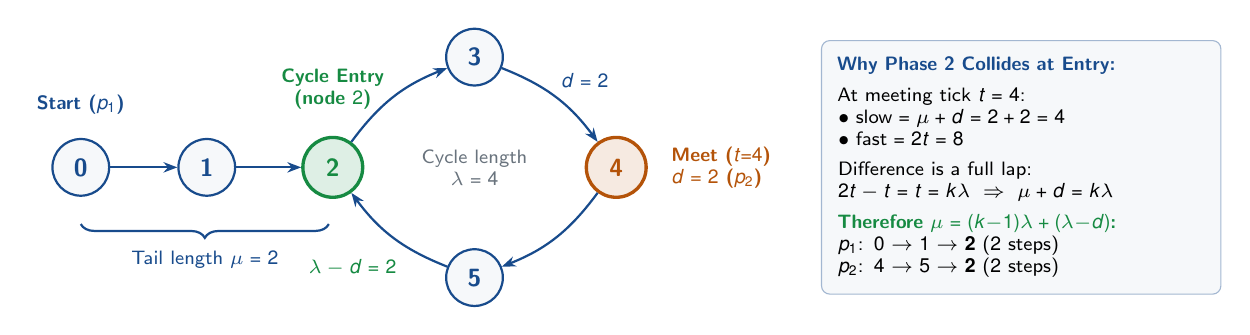
\begin{tikzpicture}[
    gnode/.style={circle, draw=primaryblue, fill=codebg, thick, minimum size=0.72cm, inner sep=0pt, font=\small\bfseries, text=primaryblue},
    entrynode/.style={circle, draw=codegreen, fill=codegreen!14, very thick, minimum size=0.76cm, inner sep=0pt, font=\small\bfseries, text=codegreen},
    meetnode/.style={circle, draw=accentamber, fill=accentamber!12, very thick, minimum size=0.76cm, inner sep=0pt, font=\small\bfseries, text=accentamber}
]
    % Tail nodes: 0 -> 1 -> 2 (compact left geometry: x = 0.55 .. 3.75)
    \node[gnode] (n0) at (0.55, 2.2) {0};
    \node[gnode] (n1) at (2.15, 2.2) {1};
    \node[entrynode] (n2) at (3.75, 2.2) {2};

    % Cycle nodes: 2 -> 3 -> 4 -> 5 -> 2 (x = 3.75 .. 7.35)
    \node[gnode] (n3) at (5.55, 3.60) {3};
    \node[meetnode] (n4) at (7.35, 2.2) {4};
    \node[gnode] (n5) at (5.55, 0.80) {5};

    % Directed edges
    \draw[lmarrow] (n0) -- (n1);
    \draw[lmarrow] (n1) -- (n2);
    \draw[lmarrow, bend left=16] (n2) to (n3);
    \draw[lmarrow, bend left=16] (n3) to (n4);
    \draw[lmarrow, bend left=16] (n4) to (n5);
    \draw[lmarrow, bend left=16] (n5) to (n2);

    % Annotations on nodes (zero collision with right card)
    \node[font=\scriptsize\bfseries\color{primaryblue}, above=5pt of n0] {Start ($p_1$)};
    \node[font=\scriptsize\bfseries\color{codegreen}, above=6pt of n2, align=center] {Cycle Entry\\(node $2$)};
    \node[font=\scriptsize\bfseries\color{accentamber}, right=5pt of n4, align=left] {Meet ($t{=}4$)\\$d = 2$ ($p_2$)};

    % Tail brace mu = 2
    \draw[decorate, decoration={brace, amplitude=5pt, mirror}, thick, primaryblue]
        (0.55, 1.48) -- (3.70, 1.48)
        node[midway, below=6pt, font=\scriptsize\color{primaryblue}] {Tail length $\mu = 2$};

    % Cycle interior label
    \node[font=\scriptsize\color{codegray}, align=center] at (5.55, 2.2) {Cycle length\\$\lambda = 4$};

    % Arc labels cleanly outside curved edges
    \node[font=\scriptsize\bfseries\color{primaryblue}] at (6.95, 3.30) {$d = 2$};
    \node[font=\scriptsize\bfseries\color{codegreen}] at (4.00, 0.92) {$\lambda - d = 2$};

    % Right Explanation Card (x = 9.95 .. 14.95 -> generous gap from Meet label)
    \node[draw=primaryblue!40, fill=codebg, rounded corners=3pt, text width=4.65cm, inner sep=6pt, font=\scriptsize, anchor=west] at (9.95, 2.2) {
        \textbf{\color{primaryblue}Why Phase 2 Collides at Entry:}\\[3pt]
        At meeting tick $t = 4$:\\
        $\bullet\;\text{slow} = \mu + d = 2 + 2 = 4$\\
        $\bullet\;\text{fast} = 2t = 8$\\[3pt]
        Difference is a full lap:\\
        $2t - t = t = k\lambda \;\Rightarrow\; \mu + d = k\lambda$\\[3pt]
        \textbf{\color{codegreen}Therefore $\mu = (k{-}1)\lambda + (\lambda{-}d)$:}\\
        $p_1$: $0 \to 1 \to \mathbf{2}$ ($2$ steps)\\
        $p_2$: $4 \to 5 \to \mathbf{2}$ ($2$ steps)
    };
\end{tikzpicture}
\caption{Floyd's Tortoise and Hare on a rho-shaped functional graph ($\mu = 2$, $\lambda = 4$). Both pointers meet at $t = 4$ (node $4$), and stepping $p_1$ from $0$ and $p_2$ from $4$ at speed $1$ collides at the exact cycle entry (node $2$).}
\label{fig:floyd_cycle}
\end{figure}

\begin{watchoutbox}[Watch Out --- Do Not Offset \texttt{fast} at Start]
Both pointers \textbf{must} start at the exact same start node $0$ before entering the Phase~1 loop (use a \texttt{do-while} loop, or advance both once before testing \texttt{slow == fast}). If you initialize \texttt{slow = 0} and \texttt{fast = next[0]}, then \texttt{fast} has traveled $2t + 1$ steps instead of $2t$, which shifts the meeting offset by $1$ and breaks Phase~2 unless you compensate!
\end{watchoutbox}

\begin{tryitbox}{Edge Cases}{Stress-Testing Floyd on Degenerate Graphs}{ex5}
Verify how Floyd's Phase~1 and Phase~2 behave on three extreme inputs (assuming safe null/out-of-bounds checks on \texttt{fast} and \texttt{next[fast]}):
\begin{enumerate}[itemsep=2pt, topsep=2pt]
    \item \textbf{Pure cycle ($\mu = 0$):} $0 \to 1 \to 2 \to 0$ (head itself is the cycle entry). Where do they meet, and how many Phase~2 steps occur?
    \item \textbf{Self-loop ($\lambda = 1$):} $0 \to 1 \to 2 \to 2$. Where do they meet, and does Phase~2 return node $2$?
    \item \textbf{Acyclic path:} $0 \to 1 \to \text{null}$ (length $2$). Which check terminates Phase~1 safely without dereferencing null?
\end{enumerate}
\end{tryitbox}

% ============================================================================
\section{Sliding Window Patterns (Fixed, Variable, and Exact-$K$)}
% ============================================================================

A \textbf{sliding window} represents a contiguous subarray or substring $A[L \dots R]$ of length $R - L + 1$. Instead of recomputing a property from scratch for every subarray, you maintain a running summary (sum, character counts, distinct count, or deficit) as $R$ moves right and $L$ follows behind.

\begin{notationbox}[Symbols Used in Sliding Windows]
$W = [L, R]$ & Current inclusive window with length $\text{len} = R - L + 1$. & $0 \le L \le R < N$ \\
$K$ & Fixed window length, or allowed budget (e.g., max distinct items). & Integer $K \ge 0$ \\
$\text{freq}[c]$ & Frequency count of item or character $c$ inside $W$. & Array / hash map \\
$\text{missing}$ & Total required character deficit still absent from $W$. & Non-negative integer \\
$\text{atMost}(K)$ & Number of non-empty subarrays with metric $\le K$. & \texttt{std::int64\_t} \\
\end{notationbox}

\subsection{Fixed-Size Sliding Window ($O(N)$)}

\painbeat Computing the maximum sum (or checking anagrams) across all $N - K + 1$ subarrays of fixed length $K$ costs $O(N \cdot K)$ naively --- $2.5 \times 10^9$ additions when $N = 10^5$ and $K = 5 \times 10^4$.

\ahabeat Two consecutive windows $[R - K, R - 1]$ and $[R - K + 1, R]$ share $K - 1$ identical elements! Moving the window one slot right requires only \textbf{two $O(1)$ operations}: add the entering element $A[R]$ and subtract the exiting element $A[R - K]$.

\begin{formulabox}[Fixed-Window Incremental Update]
$$S_R \;=\; S_{R-1} + A[R] - A[R - K] \qquad (R = K, K+1, \dots, N-1).$$
\textbf{Read this as:} Build the first window $S_{K-1} = \sum_{i=0}^{K-1} A[i]$ once, then glide right in $O(1)$ per step.
\end{formulabox}

\examplebeat On $A = [2, 1, 5, 1, 3, 2]$ with $K = 3$: initial window $[0 \dots 2]$ has sum $2+1+5 = 8$. Shift to $R=3$: $8 + 1 - 2 = 7$. Shift to $R=4$: $7 + 3 - 1 = 9$ (best). Shift to $R=5$: $9 + 2 - 5 = 6$. Total work: $6$ array reads instead of $4 \times 3 = 12$.

\textbf{Fixed-Window Anagrams in $O(N)$:} To find every start index in string $S$ that is an anagram of pattern $P$ (length $K = |P|$), maintain a frequency difference array \texttt{diff[26]} and an integer \texttt{nonzero} counting how many letters currently have $\texttt{diff}[c] \ne 0$. When adding $S[R]$ and removing $S[R - K]$, update \texttt{nonzero} in $O(1)$ whenever a bucket transitions into or out of $0$. A match occurs whenever $\texttt{nonzero} = 0$ --- avoiding even a $26$-letter loop per shift!

\begin{figure}[htbp]
\centering
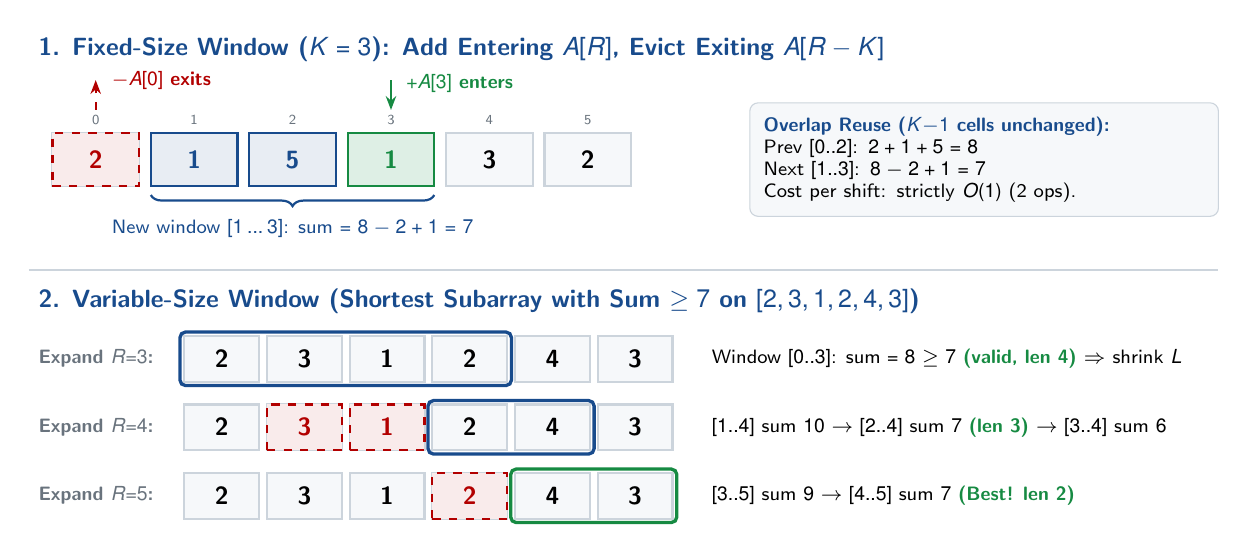
\begin{tikzpicture}[
    wcell/.style={draw=codeframe, fill=codebg, thick, minimum width=1.10cm, minimum height=0.68cm, font=\small\bfseries, inner sep=0pt, align=center}
]
    % === Top Panel: Fixed Window K = 3 on [2, 1, 5, 1, 3, 2] ===
    \node[font=\small\bfseries\color{primaryblue}, anchor=west] at (0.0, 5.95) {1. Fixed-Size Window ($K = 3$): Add Entering $A[R]$, Evict Exiting $A[R-K]$};

    % Array cells (row y = 4.55)
    \foreach \val/\i in {2/0, 1/1, 5/2, 1/3, 3/4, 2/5} {
        \node[wcell] (f\i) at (0.85 + \i*1.25, 4.55) {\val};
        \node[font=\tiny\color{codegray}] at (0.85 + \i*1.25, 5.05) {\i};
    }
    % Highlight departing f0 (red dashed), shared f1..f2 (blue), entering f3 (green)
    \node[wcell, draw=red!70!black, fill=red!70!black!8, dashed, text=red!70!black] at (0.85 + 0*1.25, 4.55) {2};
    \node[wcell, draw=primaryblue, fill=primaryblue!10, text=primaryblue] at (0.85 + 1*1.25, 4.55) {1};
    \node[wcell, draw=primaryblue, fill=primaryblue!10, text=primaryblue] at (0.85 + 2*1.25, 4.55) {5};
    \node[wcell, draw=codegreen, fill=codegreen!14, text=codegreen] at (0.85 + 3*1.25, 4.55) {1};

    % Clean top arrows for exit (-A[0]) and enter (+A[3]) so bottom brace has zero collisions
    \draw[lmprunedarrow] (0.85, 5.18) -- (0.85, 5.56) node[right=2pt, font=\scriptsize\bfseries\color{red!70!black}] {$-A[0]$ exits};
    \draw[thick, codegreen, -{Stealth[length=5pt]}] (4.60, 5.56) -- (4.60, 5.18);
    \node[font=\scriptsize\bfseries\color{codegreen}, right=2pt] at (4.60, 5.52) {$+A[3]$ enters};

    % Bracket for new window [1..3]
    \draw[decorate, decoration={brace, amplitude=4pt, mirror}, thick, primaryblue]
        (1.55, 4.10) -- (5.15, 4.10)
        node[midway, below=5pt, font=\scriptsize\color{primaryblue}] {New window $[1 \dots 3]$: sum $= 8 - 2 + 1 = 7$};

    % Right summary box for fixed window
    \node[draw=codeframe, fill=codebg, rounded corners=3pt, text width=5.6cm, inner sep=5pt, font=\scriptsize, anchor=west] at (9.15, 4.55) {
        \textbf{\color{primaryblue}Overlap Reuse ($K{-}1$ cells unchanged):}\\
        Prev $[0..2]$: $2 + 1 + 5 = 8$\\
        Next $[1..3]$: $8 - 2 + 1 = 7$\\
        Cost per shift: strictly \textbf{$O(1)$} (2 ops).
    };

    % Divider line
    \draw[codeframe, thick] (0.0, 3.15) -- (15.1, 3.15);

    % === Bottom Panel: Variable Window on [2, 3, 1, 2, 4, 3], target sum >= 7 ===
    \node[font=\small\bfseries\color{primaryblue}, anchor=west] at (0.0, 2.75) {2. Variable-Size Window (Shortest Subarray with Sum $\ge 7$ on $[2, 3, 1, 2, 4, 3]$)};

    % Step A: Expand to [0..3] sum = 8 >= 7
    \node[font=\scriptsize\bfseries\color{codegray}, anchor=west] at (0.0, 2.02) {Expand $R{=}3$:};
    \foreach \val/\i in {2/0, 3/1, 1/2, 2/3, 4/4, 3/5} {
        \node[wcell, minimum width=0.95cm, minimum height=0.58cm] at (2.45 + \i*1.05, 2.02) {\val};
    }
    \draw[primaryblue, very thick, rounded corners=2pt] (1.92, 1.68) rectangle (6.13, 2.36);
    \node[font=\scriptsize, anchor=west] at (8.55, 2.02) {Window $[0..3]$: $\text{sum} = 8 \ge 7$ \textbf{\color{codegreen}(valid, len 4)} $\Rightarrow$ shrink $L$};

    % Step B: Expand to [1..4] -> shrink twice to [3..4]
    \node[font=\scriptsize\bfseries\color{codegray}, anchor=west] at (0.0, 1.15) {Expand $R{=}4$:};
    \foreach \val/\i in {2/0, 3/1, 1/2, 2/3, 4/4, 3/5} {
        \node[wcell, minimum width=0.95cm, minimum height=0.58cm] at (2.45 + \i*1.05, 1.15) {\val};
    }
    \node[wcell, minimum width=0.95cm, minimum height=0.58cm, draw=red!70!black, fill=red!70!black!8, dashed, text=red!70!black] at (2.45 + 1*1.05, 1.15) {3};
    \node[wcell, minimum width=0.95cm, minimum height=0.58cm, draw=red!70!black, fill=red!70!black!8, dashed, text=red!70!black] at (2.45 + 2*1.05, 1.15) {1};
    \draw[primaryblue, very thick, rounded corners=2pt] (5.07, 0.81) rectangle (7.18, 1.49);
    \node[font=\scriptsize, anchor=west] at (8.55, 1.15) {$[1..4]$ sum $10 \to [2..4]$ sum $7$ \textbf{\color{codegreen}(len 3)} $\to [3..4]$ sum $6$};

    % Step C: Expand to [3..5] -> shrink to [4..5] (best len 2!)
    \node[font=\scriptsize\bfseries\color{codegray}, anchor=west] at (0.0, 0.28) {Expand $R{=}5$:};
    \foreach \val/\i in {2/0, 3/1, 1/2, 2/3, 4/4, 3/5} {
        \node[wcell, minimum width=0.95cm, minimum height=0.58cm] at (2.45 + \i*1.05, 0.28) {\val};
    }
    \node[wcell, minimum width=0.95cm, minimum height=0.58cm, draw=red!70!black, fill=red!70!black!8, dashed, text=red!70!black] at (2.45 + 3*1.05, 0.28) {2};
    \draw[codegreen, very thick, rounded corners=2pt] (6.12, -0.06) rectangle (8.23, 0.62);
    \node[font=\scriptsize, anchor=west] at (8.55, 0.28) {$[3..5]$ sum $9 \to [4..5]$ sum $7$ \textbf{\color{codegreen}(Best! len 2)}};
\end{tikzpicture}
\caption{Fixed-size vs.\ variable-size sliding windows. Fixed windows slide symmetrically in lockstep ($+A[R], -A[R-K]$), whereas variable windows expand $R$ and contract $L$ based on a monotonic validity invariant.}
\label{fig:fixed_vs_variable_window}
\end{figure}

\subsection{Variable-Size Sliding Window (Monotonic Expand \& Shrink)}

\painbeat Many problems do not give a fixed length $K$; instead they ask for the \textbf{longest} or \textbf{shortest} contiguous subarray satisfying a constraint (e.g., ``no repeated characters'', ``sum $\ge S$'', or ``contains all letters of $T$'').

\ahabeat A variable sliding window works whenever validity is \textbf{monotonic under containment}:
\begin{itemize}[itemsep=2pt, topsep=2pt]
    \item \textbf{Template A (Longest Valid Window --- Downward-Closed):} Every sub-window of a valid window is also valid (e.g., all characters unique, or sum $\le S$ with $A[i] \ge 0$). Expand $R$; \texttt{while (invalid)} shrink $L$; then record $\max(\text{best}, R - L + 1)$.
    \item \textbf{Template B (Shortest Valid Window --- Upward-Closed):} Every super-window of a valid window is also valid (e.g., sum $\ge S$ with $A[i] \ge 0$, or contains all letters of $T$). Expand $R$; \texttt{while (valid)} record $\min(\text{best}, R - L + 1)$ and shrink $L$.
\end{itemize}

\invariantbeat{Variable Window} At each $R$, Template~A finds the \emph{leftmost} $L$ making $[L, R]$ valid (maximizing length), while Template~B pushes $L$ to the \emph{rightmost} valid start for $R$ (minimizing length). Because validity is monotonic, advancing $R$ can never require $L$ to move backward.

\begin{watchoutbox}[Watch Out --- Negative Numbers Shatter Variable Sum Windows]
Template~A and Template~B \textbf{require non-negative values} ($A[i] \ge 0$) for sum constraints!
\begin{itemize}[itemsep=2pt, topsep=2pt]
    \item \textbf{Template B broken (shortest sum $\ge 3$):} On $A = [2, -1, 3]$, expanding to $R = 2$ gives $[0..2]$ with sum $4 \ge 3$ (records length $3$). Shrinking removes $A[0] = 2$, leaving $[-1, 3]$ with sum $2 < 3$, so the \texttt{while} loop stops! It \textbf{misses} the true optimal subarray $[3]$ (length $1$) because removing a positive left element lowered the sum while $-1$ was still trapped inside.
    \item \textbf{Template A broken (longest sum $\le 3$):} On $A = [4, -2, 1]$, at $R = 0$ the window $[4]$ exceeds $3$, so $L$ jumps to $1$ and permanently discards $4$. It later finds $[-2, 1]$ (length $2$), missing the full array $[4, -2, 1]$ (sum $3 \le 3$, length $3$).
\end{itemize}
\textbf{The Fix:} Whenever negative numbers appear in subarray sum problems, abandon plain sliding windows: use \textbf{Prefix Sums + Hash Map} for exact sum $= K$ (Module~04), or \textbf{Prefix Sums + Monotonic Deque} for shortest subarray with sum $\ge K$ (Module~11).
\end{watchoutbox}

\begin{tryitbox}{Trace}{Variable Window Template B}{ex6}
Trace Template~B (shortest subarray with sum $\ge 7$) on $A = [2, 3, 1, 2, 4, 3]$. Record every expand ($R$) and shrink ($L$) step, the window sum, and the updated minimum length.
\end{tryitbox}

\subsection{Counting Subarrays: The ``At Most $K$'' to ``Exactly $K$'' Trick}

\painbeat Suppose you must \emph{count} all contiguous subarrays with \textbf{exactly} $K$ distinct integers (or exactly $K$ odd numbers). Why does a single sliding window fail here?

Because ``exactly $K$'' is \textbf{not} monotonic! Shrinking $L$ can fix a window with $K + 1$ distinct elements, but once you reach $K$ distinct elements, shrinking $L$ further might \emph{keep} $K$ distinct elements (if $A[L]$ appears again later) or drop to $K - 1$. A single $L$ pointer cannot tell how many valid left endpoints exist for the current $R$.

\ahabeat Replace ``exactly $K$'' with a \emph{monotonic} constraint: \textbf{at most $K$}. If $[L, R]$ is the longest window ending at $R$ with at most $K$ distinct items, then \emph{every} suffix $[i, R]$ for $i \in \{L, L+1, \dots, R\}$ also has at most $K$ distinct items! That gives exactly $R - L + 1$ valid subarrays ending at $R$. Subtract the subarrays with at most $K - 1$ to leave \emph{only} those with exactly $K$:

\begin{formulabox}[Exact-$K$ Subarray Decomposition]
$$\text{exact}(K) \;=\; \text{atMost}(K) - \text{atMost}(K - 1), \qquad\text{where}\quad \text{atMost}(K) \;=\; \sum_{R=0}^{N-1} \bigl(R - L_K(R) + 1\bigr).$$
\textbf{Domain guard:} Define $\text{atMost}(m) = 0$ whenever $m < 0$ (and for distinct-element counting, $\text{atMost}(0) = 0$ automatically since every non-empty subarray has at least $1$ distinct element).\\
\textbf{Read this as:} Two $O(N)$ sliding-window passes give the exact count in $O(N)$ total time.
\end{formulabox}

\begin{figure}[htbp]
\centering
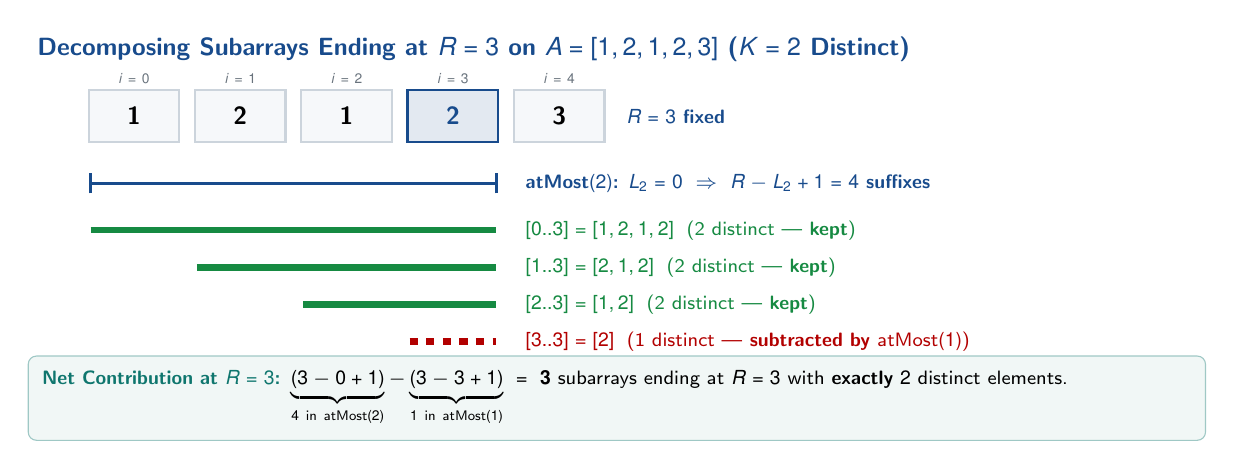
\begin{tikzpicture}[
    ecell/.style={draw=codeframe, fill=codebg, thick, minimum width=1.15cm, minimum height=0.66cm, font=\small\bfseries, inner sep=0pt, align=center}
]
    \node[font=\small\bfseries\color{primaryblue}, anchor=west] at (0.0, 4.55) {Decomposing Subarrays Ending at $R = 3$ on $A = [1, 2, 1, 2, 3]$ ($K = 2$ Distinct)};

    % Array cells
    \foreach \val/\i in {1/0, 2/1, 1/2, 2/3, 3/4} {
        \node[ecell] (e\i) at (1.35 + \i*1.35, 3.70) {\val};
        \node[font=\tiny\color{codegray}] at (1.35 + \i*1.35, 4.18) {$i=\i$};
    }
    \node[ecell, draw=primaryblue, fill=primaryblue!12, text=primaryblue] at (1.35 + 3*1.35, 3.70) {2};
    \node[font=\scriptsize\bfseries\color{primaryblue}, right=4pt of e4] {$R = 3$ fixed};

    % Bracket for atMost(2): [0..3] (4 subarrays)
    \draw[primaryblue, very thick] (0.80, 2.85) -- (5.95, 2.85);
    \draw[primaryblue, very thick] (0.80, 2.72) -- (0.80, 2.98);
    \draw[primaryblue, very thick] (5.95, 2.72) -- (5.95, 2.98);
    \node[font=\scriptsize\bfseries\color{primaryblue}, anchor=west] at (6.20, 2.85) {$\text{atMost}(2)$: $L_2 = 0 \;\Rightarrow\; R - L_2 + 1 = 4$ suffixes};

    % List the 4 suffixes visually as bars
    \draw[codegreen, line width=2.2pt] (0.80, 2.25) -- (5.95, 2.25);
    \node[font=\scriptsize\color{codegreen}, anchor=west] at (6.20, 2.25) {$[0..3] = [1,2,1,2]$ \;(2 distinct --- \textbf{kept})};

    \draw[codegreen, line width=2.2pt] (2.15, 1.78) -- (5.95, 1.78);
    \node[font=\scriptsize\color{codegreen}, anchor=west] at (6.20, 1.78) {$[1..3] = [2,1,2]$ \;(2 distinct --- \textbf{kept})};

    \draw[codegreen, line width=2.2pt] (3.50, 1.31) -- (5.95, 1.31);
    \node[font=\scriptsize\color{codegreen}, anchor=west] at (6.20, 1.31) {$[2..3] = [1,2]$ \;(2 distinct --- \textbf{kept})};

    \draw[red!70!black, line width=2.2pt, dashed] (4.85, 0.84) -- (5.95, 0.84);
    \node[font=\scriptsize\color{red!70!black}, anchor=west] at (6.20, 0.84) {$[3..3] = [2]$ \;(1 distinct --- \textbf{subtracted by }$\text{atMost}(1)$)};

    % Summary strip
    \node[draw=accentteal!40, fill=accentteal!6, rounded corners=3pt, text width=14.6cm, inner sep=5pt, font=\scriptsize, anchor=west] at (0.0, 0.12) {
        \textbf{\color{accentteal}Net Contribution at $R = 3$:}
        $\underbrace{(3 - 0 + 1)}_{4\text{ in }\text{atMost}(2)} - \underbrace{(3 - 3 + 1)}_{1\text{ in }\text{atMost}(1)} \;=\; \mathbf{3}$ subarrays ending at $R = 3$ with \textbf{exactly $2$} distinct elements.
    };
\end{tikzpicture}
\caption{Why $\text{exact}(K) = \text{atMost}(K) - \text{atMost}(K - 1)$ works: for any fixed right endpoint $R$, the valid left endpoints for ``exactly $K$'' form the exact difference between two nested suffix ranges $[L_K, R]$ and $[L_{K-1}, R]$.}
\label{fig:atmost_exact_trick}
\end{figure}

\begin{tryitbox}{Derive}{Counting Subarrays via At-Most Subtraction}{ex7}
On $A = [1, 2, 1, 2, 3]$, compute the exact number of contiguous subarrays with \textbf{exactly $K = 2$} distinct integers using $\text{atMost}(2) - \text{atMost}(1)$. Show the window start $L$ and contribution $(R - L + 1)$ for every $R = 0, 1, 2, 3, 4$ in both passes.
\end{tryitbox}

\subsection{Sliding Window vs.\ Neighboring Techniques}

Many linear-scan problems look superficially alike. Use this quick boundary check to pick the right module before writing code:

\begingroup\small\rowcolors{2}{codebg}{white}
\begin{tabularx}{\textwidth}{>{\raggedright\arraybackslash\bfseries}p{3.9cm} >{\raggedright\arraybackslash}p{4.1cm} >{\raggedright\arraybackslash}X}
\arrayrulecolor{primaryblue}\toprule[1.2pt]
\rowcolor{primaryblue!10}
\textcolor{primaryblue}{\textbf{Problem Variant}} & \textcolor{primaryblue}{\textbf{Why Sliding Window Fits / Fails}} & \textcolor{primaryblue}{\textbf{Exact Tool to Use}} \\
\arrayrulecolor{codeframe}\midrule[0.6pt]
Sum $\ge S$ / $\le S$, $A[i] \ge 0$ & Expanding increases sum; shrinking decreases sum (monotonic). & Variable Sliding Window ($O(N)$, Module~13) \\
Exact sum $= K$, negatives allowed & Sum oscillates up and down; $L$ cannot advance monotonically. & Prefix Sum + Hash Map ($O(N)$, Module~04) \\
Shortest sum $\ge S$, negatives allowed & Removing positive left elements drops sum prematurely. & Prefix Sum + Monotonic Deque ($O(N)$, Module~11) \\
Max/min element in every window of size $K$ & Evicting the old maximum leaves the second-largest unknown in $O(1)$. & Monotonic Deque ($O(N)$, Module~11) \\
Min capacity / feasibility on monotonic answer & Answer itself is monotonic (\texttt{FFFTTT}), not subarray endpoints. & Binary Search on Answer ($O(N \log R)$, Module~08) \\
\arrayrulecolor{primaryblue}\bottomrule[1.2pt]
\end{tabularx}\endgroup

\begin{tryitbox}{Triage}{Pick the Linear-Scan Tool}{ex8}
For each disguised problem ($N = 10^5$), decide whether it needs \textbf{Converging Two Pointers}, \textbf{Variable Sliding Window}, or a \textbf{Non-Window Tool (name it!)}:
\begin{enumerate}[itemsep=2pt, topsep=2pt]
    \item Given an array of positive and negative daily profits, count all contiguous periods whose total profit equals $0$.
    \item Given a binary array of $0$s and $1$s and an integer $K$, find the longest contiguous segment containing at most $K$ zeros.
    \item Given $N$ sorted package weights and a boat capacity $C$ (each boat holds at most $2$ packages), find the minimum number of boats needed.
\end{enumerate}
\end{tryitbox}

% ============================================================================
\section{Worked Examples (Paper-Reproducible Traces)}
% ============================================================================

Each example below is written so you can cover the solution and reproduce every single pointer move by hand on scratch paper.

\begin{example}[Three-Sum with Duplicate Skipping]
Find all unique triplets summing to $0$ in $A = [-2, 0, 0, 2, 2, -2, 1, -1]$.

\textbf{Step 1 --- Sort:} $A = [-2, -2, -1, 0, 0, 1, 2, 2]$ (indices $0 \dots 7$).

\textbf{Step 2 --- Fix $i$ and run converging pointers on $[i+1 \dots 7]$:}
\begin{enumerate}[itemsep=2pt, topsep=2pt]
    \item $i = 0$ ($A[0] = -2$), $L = 1, R = 7$:
    \begin{itemize}[itemsep=1pt, topsep=1pt]
        \item $(L{=}1, R{=}7)$: $-2 + (-2) + 2 = -2 < 0 \implies L \leftarrow 2$.
        \item $(L{=}2, R{=}7)$: $-2 + (-1) + 2 = -1 < 0 \implies L \leftarrow 3$.
        \item $(L{=}3, R{=}7)$: $-2 + 0 + 2 = 0 \implies$ \textbf{Record $(-2, 0, 2)$!} Move $L \leftarrow 4, R \leftarrow 6$, then skip duplicate $A[4]{=}0$ ($L \leftarrow 5$) and duplicate $A[6]{=}2$ ($R \leftarrow 5$). Now $L \ge R$, stop.
    \end{itemize}
    \item $i = 1$ ($A[1] = -2$): $A[1] = A[0]$, \textbf{skip duplicate $i$}.
    \item $i = 2$ ($A[2] = -1$), $L = 3, R = 7$:
    \begin{itemize}[itemsep=1pt, topsep=1pt]
        \item $(3, 7)$: $-1+0+2 = 1 > 0 \implies R \leftarrow 6$.
        \item $(3, 6)$: $-1+0+2 = 1 > 0 \implies R \leftarrow 5$.
        \item $(3, 5)$: $-1+0+1 = 0 \implies$ \textbf{Record $(-1, 0, 1)$!} Move $L \leftarrow 4, R \leftarrow 4$; stop ($L \ge R$).
    \end{itemize}
    \item $i = 3$ ($A[3] = 0$), $L = 4, R = 7$: $(4, 7) \to 2 > 0$, $(4, 6) \to 2 > 0$, $(4, 5) \to 1 > 0$, $R \leftarrow 4$; stop.
    \item $i = 4$ ($A[4] = 0$): $A[4] = A[3]$, \textbf{skip duplicate $i$}.
    \item $i = 5$ ($A[5] = 1 > 0$): \textbf{Early stop!} No remaining elements can sum to $0$.
\end{enumerate}
\textbf{Final Answer:} $\{(-2, 0, 2),\; (-1, 0, 1)\}$.
\end{example}

\begin{example}[Container With Most Water]
Compute the maximum water area for $h = [1, 8, 6, 2, 5, 4, 8, 3, 7]$ (indices $0 \dots 8$).

Start at $L = 0, R = 8$ and always advance whichever wall is shorter (breaking ties by \texttt{L++}):

\begingroup\footnotesize\rowcolors{2}{codebg}{white}
\begin{tabularx}{\textwidth}{>{\centering\arraybackslash}p{0.8cm} >{\centering\arraybackslash}p{1.5cm} >{\centering\arraybackslash}p{1.6cm} >{\centering\arraybackslash}p{1.1cm} >{\centering\arraybackslash}p{2.3cm} >{\centering\arraybackslash}p{1.1cm} >{\raggedright\arraybackslash}X}
\arrayrulecolor{primaryblue}\toprule[1.1pt]
\rowcolor{primaryblue!10}
\textcolor{primaryblue}{\textbf{Step}} & \textcolor{primaryblue}{\textbf{$(L, R)$}} & \textcolor{primaryblue}{\textbf{$(h[L], h[R])$}} & \textcolor{primaryblue}{\textbf{Width}} & \textcolor{primaryblue}{\textbf{Area}} & \textcolor{primaryblue}{\textbf{Best}} & \textcolor{primaryblue}{\textbf{Move (Shorter Wall)}} \\
\arrayrulecolor{codeframe}\midrule[0.6pt]
1 & $(0, 8)$ & $(1, 7)$ & $8$ & $8 \times 1 = 8$ & $8$ & $h[0] \le h[8] \implies L \leftarrow 1$ \\
2 & $(1, 8)$ & $(8, 7)$ & $7$ & $7 \times 7 = \mathbf{49}$ & $\mathbf{49}$ & $h[8] < h[1] \implies R \leftarrow 7$ \\
3 & $(1, 7)$ & $(8, 3)$ & $6$ & $6 \times 3 = 18$ & $49$ & $h[7] < h[1] \implies R \leftarrow 6$ \\
4 & $(1, 6)$ & $(8, 8)$ & $5$ & $5 \times 8 = 40$ & $49$ & $h[1] = h[6] \implies L \leftarrow 2$ \\
5 & $(2, 6)$ & $(6, 8)$ & $4$ & $4 \times 6 = 24$ & $49$ & $h[2] \le h[6] \implies L \leftarrow 3$ \\
6 & $(3, 6)$ & $(2, 8)$ & $3$ & $3 \times 2 = 6$ & $49$ & $h[3] \le h[6] \implies L \leftarrow 4$ \\
7 & $(4, 6)$ & $(5, 8)$ & $2$ & $2 \times 5 = 10$ & $49$ & $h[4] \le h[6] \implies L \leftarrow 5$ \\
8 & $(5, 6)$ & $(4, 8)$ & $1$ & $1 \times 4 = 4$ & $49$ & $h[5] \le h[6] \implies L \leftarrow 6$ (stop) \\
\arrayrulecolor{primaryblue}\bottomrule[1.1pt]
\end{tabularx}\endgroup

\textbf{Final Answer:} Maximum area is $49$ (between indices $1$ and $8$), found in $8 = N - 1$ steps instead of $\binom{9}{2} = 36$.
\end{example}

\begin{example}[Finding a Duplicate Number via Floyd's Cycle Entry]
An array of length $N + 1 = 7$ contains integers in $\{1, \dots, 6\}$ with one repeated value:
$$A = [2, 6, 4, 1, 3, 1, 5] \quad (\text{indices } 0 \dots 6).$$
Interpret $A$ as the functional graph $i \mapsto A[i]$. Since no value is $0$, node $0$ has in-degree $0$ and sits at the start of the tail, while the duplicated value ($1$, pointed to by both index $3$ and index $5$) is the \textbf{exact cycle entry}!

\textbf{Implicit path:} $0 \to 2 \to 4 \to 3 \to \mathbf{1} \to 6 \to 5 \to \mathbf{1}$ (tail $\mu = 4$, cycle $\lambda = 3$).
\begin{enumerate}[itemsep=2pt, topsep=2pt]
    \item \textbf{Phase 1 (Meet inside cycle):} Start $\text{slow} = \text{fast} = 0$.
    \begin{itemize}[itemsep=1pt, topsep=1pt]
        \item $t = 1$: $\text{slow} = A[0] = 2$, $\text{fast} = A[A[0]] = A[2] = 4$.
        \item $t = 2$: $\text{slow} = A[2] = 4$, $\text{fast} = A[A[4]] = A[3] = 1$.
        \item $t = 3$: $\text{slow} = A[4] = 3$, $\text{fast} = A[A[1]] = A[6] = 5$.
        \item $t = 4$: $\text{slow} = A[3] = 1$, $\text{fast} = A[A[5]] = A[1] = 6$.
        \item $t = 5$: $\text{slow} = A[1] = 6$, $\text{fast} = A[A[6]] = A[5] = 1$.
        \item $t = 6$: $\text{slow} = A[6] = 5$, $\text{fast} = A[A[1]] = A[6] = 5 \implies$ \textbf{Meet at node $5$!}
    \end{itemize}
    Notice $t = 6 = 2\lambda$ ($k = 2$) and offset $d = t - \mu = 6 - 4 = 2$.
    \item \textbf{Phase 2 (Locate entry):} Set $p_1 = 0$, $p_2 = 5$, advance both by $1$ step:
    \begin{itemize}[itemsep=1pt, topsep=1pt]
        \item Step 1: $(p_1, p_2) = (2, 1)$; \quad Step 2: $(4, 6)$; \quad Step 3: $(3, 5)$; \quad Step 4: $(\mathbf{1}, \mathbf{1})$!
    \end{itemize}
    Confirming $\mu = (k - 1)\lambda + (\lambda - d) = 1 \cdot 3 + (3 - 2) = 4$ steps: $p_2$ completes $1$ step to node $1$, then $1$ full lap ($1 \to 6 \to 5 \to 1$).
\end{enumerate}
\textbf{Final Answer:} Duplicate value is $\mathbf{1}$, found in $O(N)$ time and $O(1)$ space without modifying $A$.
\end{example}

\begin{example}[Minimum Window Substring (Deficit Counter)]
Find the shortest substring of $S = \texttt{"ADOBECODEBANC"}$ (indices $0 \dots 12$) containing all characters of $T = \texttt{"ABC"}$.

Initialize $\text{need}[\texttt{'A'}] = \text{need}[\texttt{'B'}] = \text{need}[\texttt{'C'}] = 1$ (all other letters $0$), and $\text{missing} = 3$. When expanding $R$, if $\text{need}[S[R]] > 0$ decrement \texttt{missing}, then always decrement $\text{need}[S[R]]$. While $\text{missing} = 0$, record the window, increment $\text{need}[S[L]]$, and if $\text{need}[S[L]] > 0$ increment \texttt{missing}.

\begingroup\footnotesize\rowcolors{2}{codebg}{white}
\begin{tabularx}{\textwidth}{>{\raggedright\arraybackslash}p{2.3cm} >{\raggedright\arraybackslash}p{3.0cm} >{\centering\arraybackslash}p{1.3cm} >{\raggedright\arraybackslash}X}
\arrayrulecolor{primaryblue}\toprule[1.1pt]
\rowcolor{primaryblue!10}
\textcolor{primaryblue}{\textbf{Phase / $R$}} & \textcolor{primaryblue}{\textbf{Valid Window $[L..R]$}} & \textcolor{primaryblue}{\textbf{Length}} & \textcolor{primaryblue}{\textbf{Shrink Action \& Updated Best}} \\
\arrayrulecolor{codeframe}\midrule[0.6pt]
Expand $R = 0..5$ & $[0..5] = \texttt{"ADOBEC"}$ & $6$ & First valid ($\text{best} = 6$). Drop $S[0]{=}\texttt{'A'} \implies \text{missing} = 1$, $L \leftarrow 1$. \\
Expand $R = 6..10$ & $[1..10] = \texttt{"DOBECODEBA"}$ & $10$ & $\text{missing} = 0$ again! Drop \texttt{D,O,B,E,O} ($L: 1 \to 5$): at $[5..10] = \texttt{"CODEBA"}$ (len $6$), drop $S[5]{=}\texttt{'C'} \implies \text{missing} = 1$, $L \leftarrow 6$. \\
Expand $R = 11..12$ & $[6..12] = \texttt{"ODEBANC"}$ & $7$ & $\text{missing} = 0$! Drop \texttt{O} ($[7..12]$, len $6$), drop \texttt{D} ($[8..12]$, len $5$), drop \texttt{E} ($[9..12] = \texttt{"BANC"}$, \textbf{len 4, new best!}). \\
Final shrink & Drop $S[9]{=}\texttt{'B'}$ & --- & $\text{need}[\texttt{'B'}] \to 1 \implies \text{missing} = 1$, $L \leftarrow 10$. $R$ finishes. \\
\arrayrulecolor{primaryblue}\bottomrule[1.1pt]
\end{tabularx}\endgroup

\textbf{Final Answer:} \texttt{"BANC"} (indices $[9..12]$, length $4$). Notice how negative entries in \texttt{need[c]} automatically track \emph{surplus} copies (like the extra \texttt{'B'} at index $3$ when $R = 9$), so dropping a surplus copy never prematurely raises \texttt{missing}.
\end{example}

\begin{example}[Subarrays With Exactly $K = 2$ Odd Numbers]
Count all contiguous subarrays of $A = [2, 1, 2, 1, 1, 2]$ containing \textbf{exactly $K = 2$} odd numbers.

\textbf{Pass 1 --- $\text{atMost}(2)$:} Maintain \texttt{odds} in $[L, R]$; shrink while $\text{odds} > 2$.
\begin{itemize}[itemsep=1pt, topsep=2pt]
    \item $R=0\;(2)$: $L=0$, odds $=0 \implies +1$. \quad $R=1\;(1)$: $L=0$, odds $=1 \implies +2$. \quad $R=2\;(2)$: $L=0$, odds $=1 \implies +3$.
    \item $R=3\;(1)$: $L=0$, odds $=2 \implies +4$.
    \item $R=4\;(1)$: odds $=3 > 2$, shrink $L=0\;(2)$ and $L=1\;(1) \implies L=2$, odds $=2 \implies +3$.
    \item $R=5\;(2)$: $L=2$, odds $=2 \implies +4$. \quad \textbf{Total $\text{atMost}(2) = 1+2+3+4+3+4 = 17$.}
\end{itemize}

\textbf{Pass 2 --- $\text{atMost}(1)$:} Shrink while $\text{odds} > 1$.
\begin{itemize}[itemsep=1pt, topsep=2pt]
    \item $R=0,1,2$: same as above ($+1, +2, +3$).
    \item $R=3\;(1)$: odds $=2 > 1$, shrink $L=0\;(2), 1\;(1) \implies L=2$, odds $=1 \implies +2$.
    \item $R=4\;(1)$: odds $=2 > 1$, shrink $L=2\;(2), 3\;(1) \implies L=4$, odds $=1 \implies +1$.
    \item $R=5\;(2)$: $L=4$, odds $=1 \implies +2$. \quad \textbf{Total $\text{atMost}(1) = 1+2+3+2+1+2 = 11$.}
\end{itemize}

\textbf{Final Answer:} $\text{exact}(2) = 17 - 11 = \mathbf{6}$ subarrays: $[2,1,2,1]$, $[1,2,1]$, $[2,1,1]$, $[1,1]$, $[2,1,1,2]$, $[1,1,2]$.
\end{example}

% ============================================================================
\section{C++23 Implementations}
% ============================================================================

Every listing below is self-contained, compiles cleanly under \texttt{g++ -std=c++23 -Wall -Wextra}, avoids \texttt{using namespace std;}, uses \texttt{std::span}/\texttt{std::string\_view} to avoid unnecessary copies, and guards empty, zero, and overflow edge cases.

\subsection{Opposite-Direction Converging Pointers}

\textbf{How it works:} \texttt{three\_sum\_zero} sorts a working copy, skips duplicate outer anchors $A[i] = A[i - 1]$, stops early once $A[i] > 0$, and runs converging pointers on $[i+1, N-1]$ using 64-bit sums to prevent overflow. \texttt{max\_water\_area} starts at the outermost walls and discards the shorter wall each iteration in $O(N)$ time.

\begin{lstlisting}[caption={Three-Sum (with duplicate skipping) and Container With Most Water.}]
#include <algorithm>
#include <array>
#include <cstdint>
#include <span>
#include <vector>

[[nodiscard]] std::vector<std::array<int, 3>>
three_sum_zero(std::vector<int> nums) {
    std::vector<std::array<int, 3>> result;
    const std::size_t n = nums.size();
    if (n < 3) return result;

    std::ranges::sort(nums);

    for (std::size_t i = 0; i + 2 < n; ++i) {
        if (nums[i] > 0) break;  // Sorted: all remaining triplets > 0
        if (i > 0 && nums[i] == nums[i - 1]) continue;

        std::size_t left = i + 1;
        std::size_t right = n - 1;
        while (left < right) {
            const std::int64_t sum = static_cast<std::int64_t>(nums[i])
                                   + nums[left] + nums[right];
            if (sum == 0) {
                result.push_back({nums[i], nums[left], nums[right]});
                ++left;
                --right;
                while (left < right && nums[left] == nums[left - 1]) ++left;
                while (left < right && nums[right] == nums[right + 1]) --right;
            } else if (sum < 0) {
                ++left;
            } else {
                --right;
            }
        }
    }
    return result;
}

[[nodiscard]] std::int64_t max_water_area(std::span<const int> height) noexcept {
    if (height.size() < 2) return 0;

    std::size_t left = 0;
    std::size_t right = height.size() - 1;
    std::int64_t best = 0;

    while (left < right) {
        const std::int64_t width = static_cast<std::int64_t>(right - left);
        const std::int64_t h = std::min(height[left], height[right]);
        best = std::max(best, width * h);

        if (height[left] <= height[right]) {
            ++left;
        } else {
            --right;
        }
    }
    return best;
}
\end{lstlisting}

\subsection{Fast \& Slow Pointers (In-Place Dedup and Floyd's Cycle Entry)}

\textbf{How it works:} \texttt{deduplicate\_at\_most\_k} compacts a sorted \texttt{std::span} in one pass, keeping an item whenever fewer than $k$ items have been written or it differs from \texttt{nums[write - k]}. \texttt{find\_cycle\_entry} treats \texttt{next\_node} as a functional graph (where an out-of-range value marks termination) and returns \texttt{std::nullopt} if acyclic or the exact cycle entry index via Phase~1 and Phase~2.

\begin{lstlisting}[caption={In-place sorted deduplication (at most $k$ copies) and Floyd's cycle entry.}]
#include <cstddef>
#include <optional>
#include <span>

[[nodiscard]] std::size_t
deduplicate_at_most_k(std::span<int> sorted_nums, std::size_t k) noexcept {
    if (k == 0) return 0;
    std::size_t write = 0;
    for (const int x : sorted_nums) {
        if (write < k || x != sorted_nums[write - k]) {
            sorted_nums[write++] = x;
        }
    }
    return write;  // Valid prefix is sorted_nums.first(write)
}

[[nodiscard]] std::optional<std::size_t>
find_cycle_entry(std::span<const std::size_t> next_node,
                 std::size_t start = 0) noexcept {
    const std::size_t n = next_node.size();
    if (start >= n) return std::nullopt;

    auto step = [&](std::size_t u) noexcept -> std::optional<std::size_t> {
        const std::size_t v = next_node[u];
        return (v < n) ? std::optional<std::size_t>{v} : std::nullopt;
    };

    std::size_t slow = start;
    std::size_t fast = start;

    // Phase 1: Advance slow by 1 and fast by 2 until they collide or exit
    while (true) {
        const auto s1 = step(slow);
        const auto f1 = step(fast);
        if (!s1 || !f1) return std::nullopt;
        const auto f2 = step(*f1);
        if (!f2) return std::nullopt;

        slow = *s1;
        fast = *f2;
        if (slow == fast) break;
    }

    // Phase 2: Reset one pointer to start; both walk at speed 1
    std::size_t p1 = start;
    std::size_t p2 = slow;
    while (p1 != p2) {
        p1 = next_node[p1];
        p2 = next_node[p2];
    }
    return p1;
}
\end{lstlisting}

\subsection{Fixed-Size Sliding Window (Max Sum and $O(1)$-Step Anagrams)}

\textbf{How it works:} \texttt{max\_sum\_window\_k} returns \texttt{std::nullopt} if $k = 0$ or $k > N$; otherwise it computes the first window sum and shifts right in $O(1)$ per step. \texttt{find\_anagram\_starts} tracks \texttt{diff[26]} and a single \texttt{nonzero} mismatch counter so every character addition/removal runs in strictly $O(1)$ time with zero inner loops.

\begin{lstlisting}[caption={Fixed-size window maximum sum and $O(N)$ lowercase anagram search.}]
#include <algorithm>
#include <array>
#include <cstdint>
#include <optional>
#include <span>
#include <string_view>
#include <vector>

[[nodiscard]] std::optional<std::int64_t>
max_sum_window_k(std::span<const int> nums, std::size_t k) noexcept {
    if (k == 0 || k > nums.size()) return std::nullopt;

    std::int64_t window_sum = 0;
    for (std::size_t i = 0; i < k; ++i) window_sum += nums[i];

    std::int64_t best = window_sum;
    for (std::size_t r = k; r < nums.size(); ++r) {
        window_sum += nums[r];
        window_sum -= nums[r - k];
        best = std::max(best, window_sum);
    }
    return best;
}

[[nodiscard]] std::vector<std::size_t>
find_anagram_starts(std::string_view text, std::string_view pattern) {
    std::vector<std::size_t> starts;
    const std::size_t k = pattern.size();
    if (k == 0 || k > text.size()) return starts;

    std::array<int, 26> diff{};
    int nonzero = 0;

    auto adjust = [&](char ch, int delta) noexcept {
        const auto idx = static_cast<std::size_t>(ch - 'a');
        if (diff[idx] == 0) ++nonzero;
        diff[idx] += delta;
        if (diff[idx] == 0) --nonzero;
    };

    // diff[c] = count in window - count in pattern
    for (const char ch : pattern) adjust(ch, -1);
    for (std::size_t i = 0; i < k; ++i) adjust(text[i], +1);
    if (nonzero == 0) starts.push_back(0);

    for (std::size_t r = k; r < text.size(); ++r) {
        adjust(text[r], +1);      // Entering character
        adjust(text[r - k], -1);  // Exiting character
        if (nonzero == 0) starts.push_back(r - k + 1);
    }
    return starts;
}
\end{lstlisting}

\subsection{Variable-Size Sliding Windows (Templates A \& B)}

\textbf{How it works:} \texttt{longest\_unique\_substring} (Template~A) uses a 256-slot \texttt{last\_pos} table to jump \texttt{left} directly past any repeated byte in $O(1)$ without an inner loop. \texttt{min\_subarray\_len\_at\_least} (Template~B) finds the shortest non-empty subarray with sum $\ge \text{target}$ on non-negative arrays, returning \texttt{std::nullopt} if no subarray reaches the target.

\begin{lstlisting}[caption={Variable-size sliding window: longest unique substring and shortest sum $\ge S$.}]
#include <algorithm>
#include <array>
#include <cstdint>
#include <limits>
#include <optional>
#include <span>
#include <string_view>

[[nodiscard]] std::size_t
longest_unique_substring(std::string_view s) noexcept {
    // Store last seen index + 1 (0 means "not seen yet")
    std::array<std::size_t, 256> last_plus_one{};
    std::size_t left = 0;
    std::size_t best = 0;

    for (std::size_t right = 0; right < s.size(); ++right) {
        const auto byte = static_cast<unsigned char>(s[right]);
        // Only jump left forward if the previous copy lies inside [left, right]
        left = std::max(left, last_plus_one[byte]);
        last_plus_one[byte] = right + 1;
        best = std::max(best, right - left + 1);
    }
    return best;
}

[[nodiscard]] std::optional<std::size_t>
min_subarray_len_at_least(std::span<const int> non_neg_nums,
                          std::int64_t target) noexcept {
    if (non_neg_nums.empty()) return std::nullopt;
    if (target <= 0) return 1;  // Any single non-negative element >= 0 >= target

    constexpr std::size_t INF = std::numeric_limits<std::size_t>::max();
    std::size_t best = INF;
    std::size_t left = 0;
    std::int64_t sum = 0;

    for (std::size_t right = 0; right < non_neg_nums.size(); ++right) {
        sum += non_neg_nums[right];
        while (left <= right && sum >= target) {
            best = std::min(best, right - left + 1);
            sum -= non_neg_nums[left++];
        }
    }
    return (best == INF) ? std::nullopt : std::optional<std::size_t>{best};
}
\end{lstlisting}

\subsection{Minimum Window Substring and Exact-$K$ Counting}

\textbf{How it works:} \texttt{min\_window\_substring} uses a compact 256-byte deficit array \texttt{need} and \texttt{missing} count, returning a zero-copy \texttt{std::string\_view} slice into \texttt{s}. \texttt{count\_exact\_k\_distinct} implements the two-pass decomposition $\text{atMost}(k) - \text{atMost}(k - 1)$ with $O(N)$ total time and safe \texttt{k == 0} handling.

\begin{lstlisting}[caption={Minimum Window Substring (deficit counter) and Exact-$K$ distinct subarrays.}]
#include <array>
#include <cstdint>
#include <limits>
#include <span>
#include <string_view>
#include <unordered_map>

[[nodiscard]] std::string_view
min_window_substring(std::string_view s, std::string_view t) noexcept {
    if (t.empty() || t.size() > s.size()) return {};

    std::array<int, 256> need{};
    for (const char ch : t) {
        ++need[static_cast<unsigned char>(ch)];
    }

    std::size_t missing = t.size();
    std::size_t left = 0;
    std::size_t best_start = 0;
    std::size_t best_len = std::numeric_limits<std::size_t>::max();

    for (std::size_t right = 0; right < s.size(); ++right) {
        const auto rc = static_cast<unsigned char>(s[right]);
        if (need[rc] > 0) --missing;
        --need[rc];

        while (missing == 0) {
            const std::size_t len = right - left + 1;
            if (len < best_len) {
                best_len = len;
                best_start = left;
            }
            const auto lc = static_cast<unsigned char>(s[left++]);
            ++need[lc];
            if (need[lc] > 0) ++missing;
        }
    }
    return (best_len == std::numeric_limits<std::size_t>::max())
               ? std::string_view{}
               : s.substr(best_start, best_len);
}

[[nodiscard]] std::int64_t
count_at_most_k_distinct(std::span<const int> nums, std::size_t k) {
    if (k == 0 || nums.empty()) return 0;

    std::unordered_map<int, std::size_t> freq;
    freq.reserve(std::min(nums.size(), k + 1));

    std::size_t left = 0;
    std::int64_t total = 0;

    for (std::size_t right = 0; right < nums.size(); ++right) {
        ++freq[nums[right]];
        while (freq.size() > k) {
            auto it = freq.find(nums[left++]);
            if (--it->second == 0) freq.erase(it);
        }
        total += static_cast<std::int64_t>(right - left + 1);
    }
    return total;
}

[[nodiscard]] std::int64_t
count_exact_k_distinct(std::span<const int> nums, std::size_t k) {
    if (k == 0) return 0;
    return count_at_most_k_distinct(nums, k)
         - count_at_most_k_distinct(nums, k - 1);
}
\end{lstlisting}

% ============================================================================
\section{Problem Pattern Recognition}
% ============================================================================

Before reaching for two pointers or a sliding window, run this 3-step check:
\begin{enumerate}[itemsep=2pt, topsep=2pt]
    \item \textbf{What is the structure?} Are you scanning pairs $(i, j)$ (sorted or symmetric), partitioning in place, following $x \mapsto f(x)$ pointers, or querying \textbf{contiguous} subarrays/substrings?
    \item \textbf{Does monotonicity hold?} Moving a pointer must permanently eliminate options or move the constraint in one predictable direction. Check immediately for \textbf{negative numbers} in sum problems!
    \item \textbf{Does $N$ forbid $O(N^2)$?} Whenever $N \ge 10^5$, nested loops will time out --- you need $O(N)$ (sliding window / two pointers) or $O(N \log N)$ (sort + two pointers).
\end{enumerate}

\begingroup\small\rowcolors{2}{codebg}{white}
\begin{tabularx}{\textwidth}{>{\raggedright\arraybackslash}p{4.3cm} >{\raggedright\arraybackslash}X >{\raggedright\arraybackslash\bfseries}p{4.1cm}}
\arrayrulecolor{primaryblue}\toprule[1.2pt]
\rowcolor{primaryblue!10}
\textcolor{primaryblue}{\textbf{Keywords in the Problem}} & \textcolor{primaryblue}{\textbf{Plain English Meaning}} & \textcolor{primaryblue}{\textbf{Tool to Use}} \\
\arrayrulecolor{codeframe}\midrule[0.6pt]
``pair/triplet with target sum'', ``sorted array'' & Order lets one comparison kill an entire row or column. & Converging Pointers ($O(N)$ / $O(N^2)$) \\
``max area / water between two lines'', ``palindrome check'' & Extreme width shrinks inward; shorter wall is dominated. & Opposite-Direction Pointers \\
``remove duplicates / zeros in-place'', ``$O(1)$ space'' & Compact valid items into prefix $A[0 \dots w-1]$ without shifting. & Read/Write Fast \& Slow Pointers \\
``sort 3 colors in one pass'', ``3-way partition'' & Separate $<p$, $=p$, $>p$ without extra buffer. & Dutch National Flag (\texttt{lo/mid/hi}) \\
``detect cycle'', ``find cycle start'', ``duplicate in $1..N$'' & Functional graph $i \mapsto A[i]$ forms a rho ($\rho$) tail + loop. & Floyd's Tortoise \& Hare ($O(1)$ space) \\
``every subarray of size $K$'', ``all anagrams of $P$'' & Fixed width slides right by $+A[R]$ and $-A[R-K]$. & Fixed Sliding Window ($O(N)$) \\
``longest substring without repeats / at most $K$ flips'' & Expanding can break validity; shrinking restores it. & Variable Window Template~A \\
``shortest subarray with sum $\ge S$ ($A[i] \ge 0$)'' & Expanding restores validity; shrink as far as possible. & Variable Window Template~B \\
``smallest substring containing all chars of $T$'' & Track character requirements with a single \texttt{missing} deficit. & Deficit Variable Window \\
``count subarrays with \emph{exactly} $K$ distinct / odds'' & Subtract two monotonic suffix counts. & $\text{atMost}(K) - \text{atMost}(K{-}1)$ \\
\arrayrulecolor{primaryblue}\bottomrule[1.2pt]
\end{tabularx}\endgroup

% ============================================================================
\section{Summary and Complexity Reference}
% ============================================================================

\begingroup\small\rowcolors{2}{codebg}{white}
\begin{tabularx}{\textwidth}{>{\raggedright\arraybackslash\bfseries}p{4.3cm} >{\centering\arraybackslash}p{2.0cm} >{\centering\arraybackslash}p{1.8cm} >{\raggedright\arraybackslash}X}
\arrayrulecolor{primaryblue}\toprule[1.2pt]
\rowcolor{primaryblue!10}
\textcolor{primaryblue}{\textbf{Task / Operation}} & \textcolor{primaryblue}{\textbf{Time}} & \textcolor{primaryblue}{\textbf{Space}} & \textcolor{primaryblue}{\textbf{Use When}} \\
\arrayrulecolor{codeframe}\midrule[0.6pt]
Sorted Pair Sum & $O(N)$ & $O(1)$ & Input is already sorted ($O(N \log N)$ if sorting first). \\
Three-Sum (Unique Triplets) & $O(N^2)$ & $O(1)^*$ & Finding unique triplets without hash-set overhead. \\
Container With Most Water & $O(N)$ & $O(1)$ & Maximizing $(R - L)\min(h[L], h[R])$ on unsorted heights. \\
In-Place Dedup / Partition & $O(N)$ & $O(1)$ & Filtering, keeping $\le k$ copies, or 3-way Dutch Flag. \\
Floyd's Cycle Detection \& Entry & $O(\mu + \lambda)$ & $O(1)$ & Linked list or $i \mapsto A[i]$ duplicate/cycle in $O(1)$ RAM. \\
Fixed-Size Window Sum & $O(N)$ & $O(1)$ & Running sum/average over every length-$K$ slice. \\
Fixed-Size Anagram Search & $O(N + \Sigma)$ & $O(\Sigma)$ & Finding all permutations of $P$ in $S$ via \texttt{nonzero}. \\
Variable Window (Templates A/B) & $O(N)$ & $O(1)$ / $O(\Sigma)$ & Longest/shortest valid contiguous slice (monotonic!). \\
Minimum Window Substring & $O(N + M)$ & $O(\Sigma)$ & Shortest slice of $S$ ($N$) covering multiset $T$ ($M$). \\
Exact-$K$ Subarray Count & $O(N)$ & $O(K)$ & Counting subarrays with exactly $K$ distinct/odd items. \\
\arrayrulecolor{primaryblue}\bottomrule[1.2pt]
\end{tabularx}\endgroup

\noindent{\footnotesize\color{codegray}$^*$In-place sorting uses $O(\log N)$ auxiliary stack space; output storage is excluded.}

% ============================================================================
\section{Glossary}
% ============================================================================

\subsection*{Core Concepts}
\begin{itemize}[itemsep=2pt]
    \item \textbf{Two Pointers}: Maintaining two array/list indices whose monotonic motion eliminates inner rescans, reducing $O(N^2)$ loops to $O(N)$.
    \item \textbf{Converging (Opposite-Direction) Pointers}: Indices $L$ and $R$ starting at $0$ and $N-1$ and walking inward while eliminating rows, columns, or dominated walls.
    \item \textbf{Fast \& Slow Pointers}: Two same-direction indices moving at different speeds or roles (read/write compaction, or $1\times$/$2\times$ cycle detection).
    \item \textbf{Loop Invariant}: A statement that holds before and after every loop iteration, proving correctness without guessing edge cases.
    \item \textbf{Amortized $O(N)$ Potential}: Proving a nested \texttt{while} loop is linear because each pointer advances monotonically at most $N$ times across the entire run.
    \item \textbf{Sliding Window}: A contiguous subarray $A[L \dots R]$ whose running summary updates incrementally as $R$ expands and $L$ contracts.
    \item \textbf{Monotonic Window Property}: Validity must be preserved either under shrinking (Template~A, downward-closed) or under expanding (Template~B, upward-closed).
    \item \textbf{Deficit Counter (\texttt{missing})}: A single integer tracking how many required items are still absent from the window, avoiding $O(\Sigma)$ map comparisons per step.
    \item \textbf{At-Most Decomposition}: Computing $\text{exact}(K) = \text{atMost}(K) - \text{atMost}(K - 1)$ when ``exact'' is non-monotonic but ``at most'' is monotonic.
    \item \textbf{Functional Graph}: A directed graph where every vertex has out-degree at most $1$ ($x \mapsto f(x)$); every finite path ends at null or enters a $\rho$-shaped tail-plus-cycle.
\end{itemize}

\subsection*{Mathematical Symbols}
\begin{itemize}[itemsep=2pt]
    \item $L, R$: Inclusive left and right boundaries of a pointer pair or sliding window $W = [L, R]$ of length $R - L + 1$.
    \item $r, w$: Fast read cursor and slow write cursor in in-place compaction ($0 \le w \le r \le N$).
    \item $\text{low}, \text{mid}, \text{high}$: Three-way partition boundaries in the Dutch National Flag algorithm.
    \item $T, S, K$: Target pair sum ($T$), threshold sum ($S$), and fixed window size or budget ($K$).
    \item $\mu, \lambda$: Tail length before a cycle ($\mu \ge 0$) and cycle period length ($\lambda \ge 1$) in Floyd's algorithm.
    \item $\text{area}(L, R)$: Water container area $(R - L) \cdot \min(h[L], h[R])$.
    \item $\text{atMost}(K),\; \text{exact}(K)$: Number of non-empty subarrays with metric $\le K$ vs.\ $= K$.
    \item $\text{freq}[c],\; \Sigma$: Frequency of symbol $c$ inside the current window, and alphabet size $\Sigma$ (e.g., $26$ or $256$).
\end{itemize}

% ============================================================================
\section{Further Reading}
% ============================================================================

\subsection*{Free Online Resources (Start Here)}
\begin{itemize}
    \item \textbf{CP-Algorithms} (\texttt{cp-algorithms.com}) --- Detailed articles on Floyd's cycle-finding algorithm, sliding-window techniques, and amortized two-pointer analysis.
    \item \textbf{Art of Problem Solving Wiki} (\texttt{artofproblemsolving.com/wiki}) --- Background on the Pigeonhole Principle (why an array of $N+1$ values in $\{1 \dots N\}$ guarantees a duplicate cycle) and modular arithmetic.
    \item \textbf{Brilliant.org} (\texttt{brilliant.org}) --- Interactive visual lessons on loop invariants, amortized analysis, and linear-time array scanning.
    \item \textbf{Project Euler} (\texttt{projecteuler.net}) --- Try \textbf{Problem 8} (Largest Product in a Series --- fixed-size sliding window with zero-reset handling) and \textbf{Problem 50} (Consecutive Prime Sum --- prefix sums / sliding window over primes).
\end{itemize}

\subsection*{Books (When You Are Ready to Go Deeper)}
\begin{itemize}
    \item \textbf{A.\ Laaksonen, \emph{Guide to Competitive Programming}} --- \emph{Beginner--Intermediate.} Clear chapter on Two Pointers, Subarray Sum, and 2-Sum/3-Sum with clean C++ walkthroughs.
    \item \textbf{S.\ Halim and F.\ Halim, \emph{Competitive Programming}} --- \emph{Intermediate.} Covers cycle finding (Floyd's and Brent's algorithms) and linear-scan window reductions.
    \item \textbf{T.\ H.\ Cormen et al., \emph{Introduction to Algorithms} (CLRS)} --- \emph{Advanced.} Rigorous treatment of loop invariants and amortized potential functions (Chapter~17).
\end{itemize}

% ============================================================================
\section*{Practice Sheet: Mixed Pen-and-Paper Drills}
\addcontentsline{toc}{section}{Practice Sheet: Mixed Pen-and-Paper Drills}
\markboth{Practice Sheet: Mixed Pen-and-Paper Drills}{}
% ============================================================================

Work through these six cold-start drills on scratch paper without looking back at the subsections. Every mode from the chapter is represented.

\begin{tryitbox}{Debug}{Negative-Number Window Failure}{ex9}
A programmer runs Variable Window Template~B (shortest subarray with sum $\ge 3$) on $A = [2, -1, 3]$.
\begin{enumerate}[itemsep=2pt, topsep=2pt]
    \item Trace the exact values of $L$, $R$, \texttt{sum}, and \texttt{best} at $R = 0, 1, 2$.
    \item What wrong answer does Template~B return, what is the true answer, and which data structure fixes this problem when negatives are allowed?
\end{enumerate}
\end{tryitbox}

\begin{tryitbox}{Twist}{Longest Substring With At Most $K$ Character Replacements}{ex10}
You may replace at most $K = 1$ character in $S = \texttt{"AABABBA"}$ to form the longest contiguous substring of identical letters. A window $[L, R]$ is valid if $(R - L + 1) - \max_{c} \text{freq}[c] \le K$. Trace Template~A on \texttt{"AABABBA"} ($K = 1$) and find the maximum length.
\end{tryitbox}

\begin{tryitbox}{Edge Cases}{Four Classic Boundary Killers}{ex11}
State the exact output (or guard needed) for each extreme input:
\begin{enumerate}[itemsep=1pt, topsep=2pt]
    \item Fixed-size window maximum sum with $N = 4$ and $K = 5$ (or $K = 0$).
    \item Three-Sum on $A = [0, 0, 0, 0, 0]$ --- how many triplets must be returned?
    \item Exact-$K$ distinct subarrays when $K = 0$ vs.\ when $K > N$.
    \item Minimum Window Substring when $S = \texttt{"a"}$ and $T = \texttt{"aa"}$.
\end{enumerate}
\end{tryitbox}

\begin{tryitbox}{Trace}{Dutch National Flag 3-Way Partition}{ex12}
Trace the 3-way Dutch National Flag partition (\texttt{low}, \texttt{mid}, \texttt{high}) on $A = [2, 0, 2, 1, 1, 0]$. Show the array and $(\text{low}, \text{mid}, \text{high})$ after every swap or advance, and explain why \texttt{mid} must \textbf{not} increment when $A[\text{mid}] = 2$.
\end{tryitbox}

\begin{tryitbox}{Derive}{Floyd's Meeting Step and Phase-2 Verification}{ex13}
Suppose a functional graph has tail length $\mu = 3$ and cycle length $\lambda = 5$: $0 \to 1 \to 2 \to 3 \to 4 \to 5 \to 6 \to 7 \to 3$.
\begin{enumerate}[itemsep=2pt, topsep=2pt]
    \item Compute the exact tick $t$ when \texttt{slow} and \texttt{fast} first meet, the meeting node, and the offset $d = t - \mu$.
    \item Verify the equation $\mu = (k - 1)\lambda + (\lambda - d)$ numerically and list the Phase~2 positions of $(p_1, p_2)$ until collision.
\end{enumerate}
\end{tryitbox}

\begin{tryitbox}{Triage}{Cold-Start Technique Selection}{ex14}
For each problem ($N = 2 \times 10^5$), name the exact technique and its time/space complexity:
\begin{enumerate}[itemsep=1pt, topsep=2pt]
    \item Given a sorted array of timestamps, count pairs $(i, j)$ with $i < j$ whose difference $A[j] - A[i] \le D$.
    \item Given an array of positive and negative integers, find the length of the longest subarray whose sum equals $T$.
    \item Given an array of positive integers, count all subarrays whose product is strictly less than $P$.
\end{enumerate}
\end{tryitbox}

% ============================================================================
\section*{Solutions to Pen-and-Paper Exercises}
\addcontentsline{toc}{section}{Solutions to Pen-and-Paper Exercises}
\markboth{Solutions to Pen-and-Paper Exercises}{}
% ============================================================================

\begin{enumerate}[itemsep=2.5pt]
    \item \label{sol:ex1}\textbf{Exercise 1 (Derive) --- Amortized Movement Budget:}
    (1) At most $N$ increments (if the condition allows $L$ to reach $R + 1 = N$; or at most $N - 1$ if $L \le R$ is kept strictly inside $[0, N-1]$). Because $L$ starts at $0$ and never decreases, total increments across the entire loop are bounded by $N$.
    (2) Resetting \texttt{R = L} on invalidation degrades runtime to $O(N^2)$: on an input where every length-$2$ window is invalid, or where validity breaks only at $R = N - 1$ for every $L$, the loop scans $\sum_{L=0}^{N-1} (N - L) = \Theta(N^2)$ elements.
    \trapnote{Assuming ``nested loop = $O(N^2)$'' without checking whether the inner index is monotonic or resets on every outer step.}

    \item \label{sol:ex2}\textbf{Exercise 2 (Trace) --- Converging Pair Sum ($T = 16$):}
    (1) $(0,5)$: $2+15=17 > 16 \implies$ kill col $5$, $R \leftarrow 4$.
    (2) $(0,4)$: $2+12=14 < 16 \implies$ kill row $0$, $L \leftarrow 1$.
    (3) $(1,4)$: $5+12=17 > 16 \implies$ kill col $4$, $R \leftarrow 3$.
    (4) $(1,3)$: $5+9=14 < 16 \implies$ kill row $1$, $L \leftarrow 2$.
    (5) $(2,3)$: $7+9=16 = T \implies$ \textbf{Match at $(2, 3)$!}
    \trapnote{Stopping at $L \le R$ instead of $L < R$, which falsely pairs an element with itself ($A[i] + A[i] = T$).}

    \item \label{sol:ex3}\textbf{Exercise 3 (Debug) --- Breaking Neighbor-Peek Heuristic:}
    (1) On $[1, 2, 10, 10, 1]$: start $(0, 4)$ area $4 \cdot 1 = 4$. Neighbors are $h[1] = 2$ vs.\ $h[3] = 10$, so the buggy rule moves $R \leftarrow 3$ (area $3 \cdot 1 = 3$). Next $h[1] = 2$ vs.\ $h[2] = 10$, so it moves $R \leftarrow 2$ (area $2 \cdot 1 = 2$). Next $h[1] = 2$ vs.\ $h[1] = 2$, tie breaks to $R \leftarrow 1$ (area $1 \cdot 1 = 1$). It reports \textbf{$4$}.
    (2) True optimum is $(2, 3)$ with area $1 \cdot 10 = \mathbf{10}$. The shorter-wall rule moves $L \to 1 \to 2$ while keeping tall $h[3]=10$, hitting $(2, 3)$.
    \trapnote{Peeking one step ahead can trap you forever on a tiny outer wall ($h[0] = 1$) while throwing away the tall right wall ($h[3] = 10$).}

    \item \label{sol:ex4}\textbf{Exercise 4 (Twist) --- Keep At Most Two Copies:}
    $r=0\;(1)$: $w<2 \Rightarrow [1], w=1$.
    $r=1\;(1)$: $w<2 \Rightarrow [1,1], w=2$.
    $r=2\;(1)$: $A[2] = A[0] = 1 \Rightarrow$ skip ($w=2$).
    $r=3\;(2)$: $2 \ne A[1]{=}1 \Rightarrow [1,1,2], w=3$.
    $r=4\;(2)$: $2 \ne A[2]{=}1 \Rightarrow [1,1,2,2], w=4$.
    $r=5\;(3)$: $3 \ne A[3]{=}2 \Rightarrow [1,1,2,2,3], w=5$. Final prefix: $[1, 1, 2, 2, 3]$, length $w = 5$.
    \trapnote{Comparing $A[r]$ against $A[r - 2]$ instead of $A[w - 2]$: once elements are overwritten, $A[r - 2]$ no longer reflects the compacted output!}

    \item \label{sol:ex5}\textbf{Exercise 5 (Edge Cases) --- Degenerate Floyd Graphs:}
    (1) Pure cycle ($\mu = 0, \lambda = 3$): $t=1:(1,2)$, $t=2:(2,1)$, $t=3:(0,0)$ --- meet at node $0$; Phase~2 checks $p_1 = p_2 = 0$ immediately ($0$ steps) and returns $0$.
    (2) Self-loop ($\mu = 2, \lambda = 1$): $t=1:(1,2)$, $t=2:(2,2)$ --- meet at node $2$; Phase~2 steps $(0,2) \to (1,2) \to (2,2)$ ($2$ steps) and returns $2$.
    (3) Acyclic $0 \to 1 \to \text{null}$: at $t = 1$, \texttt{fast} steps $0 \to 1 \to \text{null}$; checking \texttt{f1} and \texttt{f2} before dereferencing exits cleanly with \texttt{std::nullopt}.
    \trapnote{Testing \texttt{while (slow != fast)} before taking the first step exits immediately at $t = 0$ because both pointers start at $0$.}

    \item \label{sol:ex6}\textbf{Exercise 6 (Trace) --- Variable Window Template B ($S = 7$):}
    $R=0..2$: sums $2, 5, 6 < 7$.
    $R=3\;(2)$: $[0..3]$ sum $8 \ge 7$ (best $= 4$), shrink $L=0\;(-2) \Rightarrow$ sum $6, L=1$.
    $R=4\;(4)$: $[1..4]$ sum $10 \ge 7$ (best $= 4$), shrink $L=1\;(-3) \Rightarrow [2..4]$ sum $7 \ge 7$ (best $= 3$), shrink $L=2\;(-1) \Rightarrow$ sum $6, L=3$.
    $R=5\;(3)$: $[3..5]$ sum $9 \ge 7$ (best $= 3$), shrink $L=3\;(-2) \Rightarrow [4..5]$ sum $7 \ge 7$ (\textbf{best $= 2$}), shrink $L=4\;(-4) \Rightarrow$ sum $3, L=5$. Final answer: $\mathbf{2}$ ($[4, 3]$).
    \trapnote{Recording \texttt{best} \emph{after} the \texttt{while} loop (like Template~A) instead of \emph{inside} it --- after the loop terminates, the window is no longer valid!}

    \item \label{sol:ex7}\textbf{Exercise 7 (Derive) --- Exact-$2$ Distinct on $[1, 2, 1, 2, 3]$:}\\
    $\text{atMost}(2)$ triples $(R, L, R{-}L{+}1)$: $(0,0,1)$, $(1,0,2)$, $(2,0,3)$, $(3,0,4)$, $(4,3,2)$ $\implies$ sum $= 12$.\\
    $\text{atMost}(1)$ triples $(R, L, R{-}L{+}1)$: $(0,0,1)$, $(1,1,1)$, $(2,2,1)$, $(3,3,1)$, $(4,4,1)$ $\implies$ sum $= 5$.\\
    Therefore $\text{exact}(2) = 12 - 5 = \mathbf{7}$ subarrays.
    \trapnote{Forgetting to erase a key from the frequency map when its count drops to $0$, which leaves \texttt{freq.size()} permanently inflated.}

    \item \label{sol:ex8}\textbf{Exercise 8 (Triage) --- Linear-Scan Tool Selection:}
    (1) \textbf{Prefix Sum + Hash Map} (Module~04) --- negative values break sliding-window monotonicity.
    (2) \textbf{Variable Sliding Window Template~A} --- count zeros in $[L, R]$ and shrink $L$ while $\text{zeros} > K$.
    (3) \textbf{Converging Two Pointers} (greedy matching, Module~10 + 13) --- pair lightest $A[L]$ with heaviest $A[R]$ if $A[L]+A[R] \le C$; else ship $A[R]$ alone.
    \trapnote{Reaching for a sliding window on Problem~1 just because it says ``contiguous periods'' --- always check whether negative values exist first.}

    \item \label{sol:ex9}\textbf{Exercise 9 (Debug) --- Negative-Number Window Failure:}
    (1) $R=0$: $[0..0]$ sum $2 < 3$. $R=1$: $[0..1]$ sum $1 < 3$. $R=2$: $[0..2]$ sum $4 \ge 3 \Rightarrow \text{best} = 3$; shrink $L=0\;(-2) \Rightarrow [1..2]$ sum $2 < 3$, \texttt{while} stops!
    (2) Template~B returns \textbf{$3$} instead of the true optimum \textbf{$1$} ($[3]$). Fix: \textbf{Prefix Sums + Monotonic Deque} (Module~11).
    \trapnote{Testing your sliding-window solution only on positive sample inputs and missing that $-1$ traps $L$ behind a valid shorter suffix.}

    \item \label{sol:ex10}\textbf{Exercise 10 (Twist) --- Longest Repeating Character Replacement:}
    $R=0\;(A)$: $L=0$, $\max f = 1$, len $1$. $R=1\;(A)$: $\max f = 2$, len $2$. $R=2\;(B)$: $3-2 \le 1$, len $3$. $R=3\;(A)$: \texttt{"AABA"}, $\max f = 3$, $4-3 \le 1$, \textbf{best $= 4$}.
    $R=4\;(B)$: $5-3 > 1 \Rightarrow L=1$ (\texttt{"ABAB"}, len $4$). $R=5\;(B)$: $5-3 > 1 \Rightarrow L=2$ (\texttt{"BABB"}, len $4$). $R=6\;(A)$: $5-3 > 1 \Rightarrow L=3$ (\texttt{"ABBA"}, len $4$). Final answer: $\mathbf{4}$.
    \trapnote{Recomputing $\max f$ over all $26$ letters works in $O(26N)$, or you can keep the historical maximum $\max f$ because shrinking the window below the best length already seen can never produce a new record.}

    \item \label{sol:ex11}\textbf{Exercise 11 (Edge Cases) --- Four Boundary Killers:}
    (1) Both $K > N$ and $K = 0$ have no valid length-$K$ subarray $\implies$ return \texttt{std::nullopt} (never loop \texttt{0..k-1} without checking $k \le N$).
    (2) Exactly \textbf{one} unique triplet: $(0, 0, 0)$ (all duplicate $i, L, R$ values are skipped).
    (3) Both return $\mathbf{0}$ (no non-empty subarray has $0$ or $> N$ distinct items); guard $k = 0$ before computing $k - 1$ to prevent unsigned underflow!
    (4) Returns empty string \texttt{""} because $|T| > |S|$ (or \texttt{missing} never hits $0$).
    \trapnote{Computing \texttt{k - 1} on an unsigned \texttt{std::size\_t k = 0} wraps around to $2^{64} - 1$ and causes an infinite-budget bug.}

    \item \label{sol:ex12}\textbf{Exercise 12 (Trace) --- Dutch National Flag on $[2, 0, 2, 1, 1, 0]$:}
    Start $(\text{lo}, \text{mid}, \text{hi}) = (0, 0, 5)$:
    (1) $A[0]=2 \Rightarrow \text{swap}(0,5), \text{hi}\leftarrow 4$: $[0,0,2,1,1,2]$, $(0,0,4)$.
    (2) $A[0]=0 \Rightarrow \text{swap}(0,0), \text{lo}\leftarrow 1, \text{mid}\leftarrow 1$: $(1,1,4)$.
    (3) $A[1]=0 \Rightarrow \text{swap}(1,1), \text{lo}\leftarrow 2, \text{mid}\leftarrow 2$: $(2,2,4)$.
    (4) $A[2]=2 \Rightarrow \text{swap}(2,4), \text{hi}\leftarrow 3$: $[0,0,1,1,2,2]$, $(2,2,3)$.
    (5) $A[2]=1 \Rightarrow \text{mid}\leftarrow 3$: $(2,3,3)$.
    (6) $A[3]=1 \Rightarrow \text{mid}\leftarrow 4 > \text{hi} \Rightarrow$ done: $[0, 0, 1, 1, 2, 2]$.
    \texttt{mid} stays put after swapping with \texttt{high} because the incoming value $A[\text{high}]$ was unclassified (notice in Step~1 a $0$ arrived at index $0$!).
    \trapnote{Incrementing \texttt{mid} in the $A[\text{mid}] = 2$ branch leaves that freshly swapped $0$ permanently stranded in the middle $1$s region.}

    \item \label{sol:ex13}\textbf{Exercise 13 (Derive) --- Floyd's Meeting Step ($\mu = 3, \lambda = 5$):}
    (1) $t=1:(1,2)$, $t=2:(2,4)$, $t=3:(3,6)$, $t=4:(4,3)$, $t=5:(5,5)$ $\implies$ meet at tick $t = \mathbf{5}$, node $\mathbf{5}$, with offset $d = t - \mu = 5 - 3 = \mathbf{2}$.
    (2) Here $t = 5 = 1 \cdot \lambda$ ($k = 1$), so $(k-1)\lambda + (\lambda - d) = 0 \cdot 5 + (5 - 2) = 3 = \mu$. Phase~2: $(0, 5) \to (1, 6) \to (2, 7) \to (\mathbf{3}, \mathbf{3})$ after $3$ steps!
    \trapnote{Assuming $t$ always equals $\mu + \lambda$; actually $t$ is the smallest multiple of $\lambda$ that is $\ge \mu$, namely $t = \lceil \mu / \lambda \rceil \cdot \lambda$ (or $\lambda$ when $\mu = 0$).}

    \item \label{sol:ex14}\textbf{Exercise 14 (Triage) --- Cold-Start Selection:}
    (1) \textbf{Same-Direction Sliding Window} on the sorted array: for each $R$, advance $L$ while $A[R] - A[L] > D$, then add $R - L$ pairs ($O(N)$ time, $O(1)$ space).
    (2) \textbf{Prefix Sum + Hash Map} storing the \emph{earliest} index of each prefix sum ($O(N)$ time, $O(N)$ space) --- negatives break sliding windows.
    (3) \textbf{Variable Sliding Window Template~A} (all values $> 0$, so product is monotonic!): shrink $L$ while $\text{prod} \ge P$, then add $R - L + 1$ ($O(N)$ time, $O(1)$ space; guard $P \le 1 \Rightarrow 0$).
    \trapnote{Using opposite-direction pointers on Problem~1 when it asks for a \emph{difference} $A[j] - A[i] \le D$: differences require same-direction pointers so advancing $R$ increases the difference and advancing $L$ decreases it.}
\end{enumerate}

% ============================================================================
\section*{Version History}
\addcontentsline{toc}{section}{Version History}
\markboth{Version History}{}
% ============================================================================

\begin{center}
\begingroup
\small
\rowcolors{2}{codebg}{white}
\begin{tabularx}{\textwidth}{>{\bfseries}l >{\raggedright\arraybackslash}X}
\arrayrulecolor{primaryblue}\toprule[1.2pt]
\rowcolor{primaryblue!10}
\textcolor{primaryblue}{\textbf{Date}} & \textcolor{primaryblue}{\textbf{Change}} \\
\arrayrulecolor{codeframe}\midrule[0.6pt]
2026-11-26 & Document created. \\
\arrayrulecolor{primaryblue}\bottomrule[1.2pt]
\end{tabularx}
\endgroup
\end{center}

\end{document}
